\documentclass[11pt]{article}

% "review" produces the anonymous, line-numbered version required by ARR.
\usepackage[review]{acl}

\usepackage{times}
\usepackage{latexsym}
\usepackage[T1]{fontenc}
\usepackage[utf8]{inputenc}
\usepackage{microtype}
\usepackage{graphicx}
\usepackage{amsmath,amssymb,amsthm}
\usepackage{booktabs}
\usepackage{multirow}
\usepackage{pifont}
\usepackage{enumitem}
\usepackage{eso-pic}
\usepackage{tikz}
\usetikzlibrary{positioning,arrows.meta,calc}
\usepackage{pgfplots}
\pgfplotsset{compat=1.17}

% ======================================================================
% PLACEHOLDER MACHINERY
% Every number that must come from an experiment is written as \ph{...}.
% While \placeholderstrue is set, such numbers print in red, each page
% carries a red draft banner, and Appendix A states the draft status.
% Switching to \placeholdersfalse makes any remaining \ph{...} a compile
% ERROR, so the paper cannot be built for submission until every
% placeholder has been replaced by a measured value (typed without \ph).
% ======================================================================
\newif\ifplaceholders
\placeholderstrue
\newcommand{\ph}[1]{%
  \ifplaceholders\textcolor{red}{#1}%
  \else\PackageError{draft}{Placeholder value `#1' has not been replaced}%
       {Replace every \string\ph{...} by a measured number before submission.}%
  \fi}
\newcommand{\phmark}{\ifplaceholders
  \node[red, font=\tiny\bfseries, rotate=14, opacity=0.5]
     at (rel axis cs:0.5,0.5) {PLACEHOLDER DATA};\fi}
\ifplaceholders
\AddToShipoutPictureBG{\AtPageUpperLeft{\raisebox{-0.9cm}{\hspace{2.2cm}%
  \textcolor{red}{\footnotesize\sffamily DRAFT v13. Black numbers in results are
  measured at seed 0 and provisional. Red is a placeholder, not a measurement. Not for submission
  in this state.}}}}
\fi

% ======================================================================
% MEASURED NUMBERS
% \res{key} prints a value that scripts/make_tables.py computed from the
% result files and wrote to numbers.tex (keys: docstring of make_tables.py).
% A key without a measured value prints \ph{tbd}. Table and figure bodies
% between "% <tables:name>" and "% </tables:name>" are replaced from
% tables/<name>.tex by scripts/update_paper.py; do not edit them by hand.
% ======================================================================
\makeatletter
\newcommand{\resdef}[2]{\@namedef{res@#1}{#2}}
\newcommand{\res}[1]{\@ifundefined{res@#1}{\ph{tbd}}{\@nameuse{res@#1}}}
\makeatother
\newcommand{\sd}[1]{\,{\scriptsize$\pm$#1}}
\InputIfFileExists{numbers.tex}{}{}

% ---------- shorthands ----------
\newcommand{\method}{Ledger-RM}
\newcommand{\cmark}{\ding{51}}
\newcommand{\xmark}{\ding{55}}
\newcommand{\up}{$\uparrow$}
\newcommand{\dn}{$\downarrow$}
\newcommand{\xf}{x^{\mathrm{f}}}
\newcommand{\xn}{x^{\mathrm{n}}}
\newcommand{\xm}{x^{\mathrm{m}}}
\newcommand{\xp}{x^{\mathrm{p}}}
\newcommand{\bb}{Qwen3.5-9B}
\newtheorem{proposition}{Proposition}
\setlist{nosep,leftmargin=*}

\title{Learning When to Change: Symbolic Supervision for\\
Selective Evidence Sensitivity in Medical Reward Models}

\author{Anonymous ACL submission}

\begin{document}
\maketitle

\begin{abstract}
Reward models decide which medical reasoning traces are kept, reranked and
reinforced. A useful reward reverses its preference when decisive patient
evidence changes and holds it when similar-looking evidence does not apply: a
penicillin allergy in the patient is a reason to change an order, the same
allergy in the patient's mother is not. We test this \emph{selective
sensitivity} with symbolic triplets from executable, stated clinical rules: a
base case, a flip of one decisive input, and a near-miss that mentions the
same concept without making it applicable. Labels state compliance with the
rule shown, not clinical optimality. Across \ph{13} reward signals,
\ph{14}--\ph{75}\% of triplets are solved: trained medical PRMs seldom
reverse, and general judges reverse on near-misses. Training on flip pairs
alone leaves this over-triggering unresolved, and near-misses in the same
budget remove most of it. A reader that records each finding with its
subject, status and time, followed by a judge with no direct access to the
case, solves \ph{99}\% of triplets on rules of held-out structure,
\ph{1.2} points more than an evidence summary in prose under the same
two-stage interface. Trained on rules alone, with no medical QA data, the
model raises agreement with MedEinst pair labels from \ph{18}\% to
\ph{45}\% and macro-F1 against physician-annotated eligibility judgments from
\ph{tbd} to \ph{tbd}. Outside rules, selectivity is tested only indirectly,
since existing clinical benchmarks contain no case edits of this kind.
\end{abstract}

\section{Introduction}

A reward model for medical reasoning is asked whether a step or an answer is
right for the patient at hand. Often the answer turns on one line of the case.
Under a rule that orders amoxicillin for streptococcal pharyngitis unless the
patient is allergic to penicillin, the order is right for a patient with no
drug allergy and wrong for one with a documented penicillin allergy
(Figure~\ref{fig:example}). It is right again for a patient whose mother has
that allergy. A reward that prefers the same order in all three cases fails to
reverse when required. One that changes its preference in the second and the
third reverses under an edit that leaves the decision unchanged. Whether
evidence applies also depends on the rule: a stroke ten years ago counts
under a score that asks for any prior stroke and not under a criterion that
asks about the last six months.

\begin{figure}[t]
\centering\footnotesize
\parbox{0.97\linewidth}{%
\textbf{Stated rule.} Strep.\ pharyngitis: order amoxicillin; if the patient is
allergic to penicillin, order azithromycin.\\
\textbf{Claims.} $s$: ``Order amoxicillin.'' \ \ $s'$: ``Order azithromycin.''}
\\[3pt]
\setlength{\tabcolsep}{3pt}
\begin{tabular}{@{}llcc@{}}
\toprule
Case & Reports & Rule & Required $d$\\
\midrule
base $x$      & allergies: none          & $s$  & $>0$\\
decisive edit $\xf$ & allergy: penicillin & $s'$ & $<0$\\
near-miss $\xn$ & mother: penicillin all. & $s$  & $>0$\\
missing $\xm$ & allergy status unknown   & --   & reject both\\
\bottomrule
\end{tabular}
\caption{One rule, four generated cases (schematic). $d=u(s)-u(s')$ is the
preference a verifier should show. A verifier that prefers $s$ throughout
fails to reverse; one that prefers $s'$ whenever the allergy is named
reverses on the near-miss.}
\label{fig:example}
\end{figure}

Both failures matter because reward models filter training traces
\citep{chen2024huatuo}, rerank candidates \citep{snell2025scaling,yun2025medprm}
and supply the reward in reinforcement learning
\citep{shao2024deepseekmath,guo2025deepseekr1}. The first is documented: LLM
judges are more reliably invariant to irrelevant edits than sensitive to
relevant ones \citep{chen2026judge}, and clinical LLMs mention a changed
patient fact in 85.6\% of their rationales while keeping the original
medication choice in 69.8\% \citep{hou2026medpic}. The second is easy to
overlook: an output change after a targeted edit means little unless it exceeds
the change after an edit that should not matter \citep{yang2026compared}.
Medical reward models are evaluated on answer selection and on injected step
errors \citep{yun2025medprm,wu2026medprmbench}, neither of which changes the
case. Training for sensitivity to relevant changes and invariance to
irrelevant ones exists for reward models \citep{srivastava2026crome}, and
labels from formal verification transfer to informal tasks
\citep{kamoi2026fover}. What is not established is what a reward learns when
the ``irrelevant'' evidence is about the very concept the rule tests, and
which supervision teaches it when that evidence applies.

We build the test from executable rules (\S\ref{sec:twins}). Each rule yields
\emph{triplets}: a base case, a \emph{decisive edit} (flip) of one input, and
a \emph{near-miss} in which the decisive concept appears without counting
under the rule: in a relative, negated, at a time the rule does not count, or
as a value that approaches a threshold without crossing it. Each case is
crossed with the two claims the rule can support, and the rule program labels
all six instances. Labels state what a stated rule implies, not what is
clinically best, and each judgment concerns one condition of one rule: the
task is local applicability verification. External benchmarks with existing
labels form further tiers, each measuring a different construct
(Table~\ref{tab:sources}).

Three things should be kept apart. A \emph{claim verifier} scores a claim
against a case; a \emph{process reward model} uses such scores to rank or
filter reasoning traces; a \emph{training reward} is optimised against by a
policy. Our triplet experiments concern the first, candidate selection
(\S\ref{sec:results-downstream}) the second, and policy training
(Appendix~\ref{app:more}) the third. A result at one level is not evidence
for the next, and we make no claim about preventing reward exploitation
beyond what the policy-training experiment measures. Our contributions:

\noindent\textbf{(1) A test.} Triplets separate two failures that pair tests
conflate, and rule-side edits change whether the same evidence counts. Across
\ph{13} reward signals \ph{13.8}--\ph{75.0}\% of triplets are solved
(\S\ref{sec:results-audit}).

\noindent\textbf{(2) A controlled comparison} of training distributions and
intermediate representations under one interface and budget
(\S\ref{sec:results-factorial}): flip pairs alone leave over-triggering
unresolved, near-misses correct it, and a typed applicability ledger is
\ph{1.2} points above a prose summary that carries the same facts and is read
by the same case-blind judge. A separately written record is what helps: the
same ledger written in one pass with the verdict gives no gain.

\noindent\textbf{(3) Transfer under named controls.} A model trained on rule
triplets only reaches \ph{99.2}\% on rules of held-out structure and, without
medical QA data, raises agreement with MedEinst labels from \ph{18.4}\% to
\ph{44.8}\% and with physician eligibility judgments from \ph{tbd} to
\ph{tbd} (\S\ref{sec:results-shift}).

\begin{figure*}[t]
\centering
\resizebox{\textwidth}{!}{%
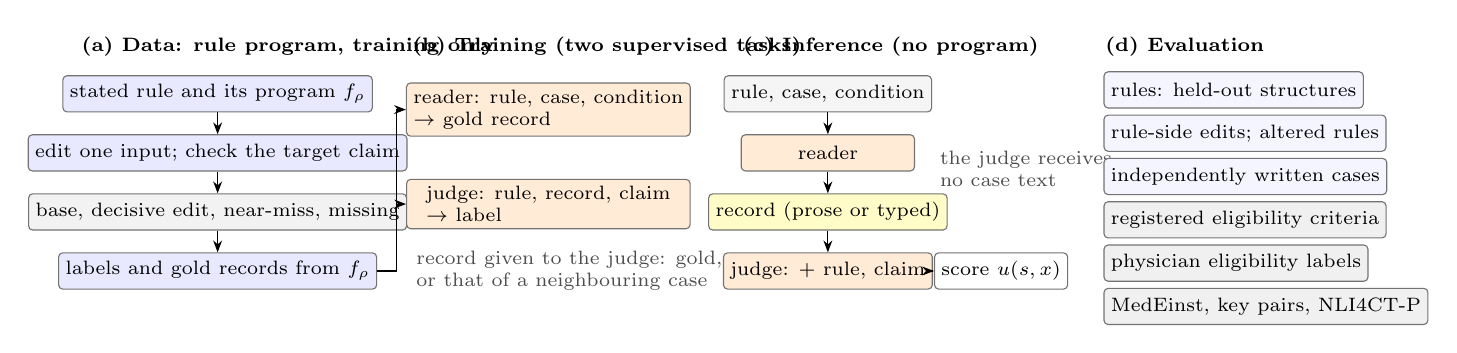
\begin{tikzpicture}[font=\scriptsize, >={Stealth[length=1.5mm]},
  box/.style={draw=black!55, rounded corners=1.5pt, align=center,
              inner sep=2.5pt, minimum height=4.6mm},
  sym/.style={box, fill=blue!9},
  neu/.style={box, fill=orange!16},
  hd/.style={font=\scriptsize\bfseries, anchor=west}]
% (a) data
\node[hd] at (-0.05,3.3) {(a) Data: rule program, training only};
\node[sym, minimum width=36mm] (rule) at (1.8,2.7) {stated rule and its program $f_\rho$};
\node[sym, minimum width=36mm] (edit) at (1.8,1.95) {edit one input; check the target claim};
\node[box, fill=black!5, minimum width=36mm] (cases) at (1.8,1.2) {base, decisive edit, near-miss, missing};
\node[sym, minimum width=36mm] (lab) at (1.8,0.45) {labels and gold records from $f_\rho$};
\draw[->] (rule) -- (edit); \draw[->] (edit) -- (cases); \draw[->] (cases) -- (lab);
% (b) training
\node[hd] at (4.15,3.3) {(b) Training (two supervised tasks)};
\node[neu, minimum width=36mm, align=left] (rt) at (6.0,2.5) {reader: rule, case, condition\\ $\rightarrow$ gold record};
\node[neu, minimum width=36mm, align=left] (jt) at (6.0,1.3) {judge: rule, record, claim\\ $\rightarrow$ label};
\node[text=black!70, align=left, anchor=west] at (4.2,0.45) {record given to the judge: gold,\\ or that of a neighbouring case};
\draw[->] (lab.east) -- ++(0.25,0) |- (rt.west);
\draw[->] (lab.east) -- ++(0.25,0) |- (jt.west);
% (c) inference
\node[hd] at (8.35,3.3) {(c) Inference (no program)};
\node[box, fill=black!4, minimum width=22mm] (inp) at (9.55,2.7) {rule, case, condition};
\node[neu, minimum width=22mm] (reader) at (9.55,1.95) {reader};
\node[box, fill=yellow!22, minimum width=22mm] (rec) at (9.55,1.2) {record (prose or typed)};
\node[neu, minimum width=22mm] (judge) at (9.55,0.45) {judge: + rule, claim};
\node[box, fill=white, minimum width=14mm] (score) at (11.75,0.45) {score $u(s,x)$};
\draw[->] (inp) -- (reader); \draw[->] (reader) -- (rec); \draw[->] (rec) -- (judge); \draw[->] (judge) -- (score);
\node[text=black!70, align=left, anchor=west] at (10.85,1.75) {the judge receives\\ no case text};
% (d) evaluation
\node[hd] at (12.95,3.3) {(d) Evaluation};
\node[box, anchor=west, fill=blue!4,  minimum width=27mm] at (13.05,2.75) {rules: held-out structures};
\node[box, anchor=west, fill=blue!4,  minimum width=27mm] at (13.05,2.2) {rule-side edits; altered rules};
\node[box, anchor=west, fill=blue!4,  minimum width=27mm] at (13.05,1.65) {independently written cases};
\node[box, anchor=west, fill=black!6, minimum width=27mm] at (13.05,1.1) {registered eligibility criteria};
\node[box, anchor=west, fill=black!6, minimum width=27mm] at (13.05,0.55) {physician eligibility labels};
\node[box, anchor=west, fill=black!6, minimum width=27mm] at (13.05,0.0) {MedEinst, key pairs, NLI4CT-P};
\end{tikzpicture}}
\caption{Overview. (a) The rule program produces cases, labels and gold
evidence records. (b) It supervises two tasks and is not used afterwards.
(c) At inference the reader writes a record from the rule, the case and the
condition under test; the judge scores the claim from the rule and the
record. A string check on quotations is the only symbolic operation.
(d) Controlled tests (blue) and external labels (grey).}
\label{fig:overview}
\end{figure*}

\section{Related Work}

\paragraph{Validity of evaluators.}
\citet{chen2026judge} define a judge's validity as invariance to
construct-preserving edits together with sensitivity to construct-changing
ones. \citet{yang2026compared} show that the effect of a targeted
counterfactual edit must be compared with that of meaning-preserving edits of
the same size; our near-miss and presentation edits are such baselines with
known labels. Robustness work on reward models targets response-side
artifacts \citep{liu2025rrm,zang2025auditor,xu2025contextualjudge}. CROME
trains reward models with augmentations that change causal attributes of a
response and with neutral augmentations that should leave the reward
unchanged \citep{srivastava2026crome}: sensitivity to relevant changes
together with invariance to irrelevant ones is established for reward
training. DynaCF uses perturbation sensitivity differently: it rewrites the
chosen response without changing its content and down-weights training pairs
whose margin shifts \citep{liu2026dynacf}; we include an adaptation of this
re-weighting to case edits as an alternative to training on near-misses. CSR
regularises a solver to change its answer when an operator in its own trace
is swapped \citep{shihab2025csr}.

\paragraph{Process rewards and symbolic supervision.}
PRMs are trained on human step labels \citep{lightman2024verify}, rollout
estimates \citep{wang2024mathshepherd} or generated verification reasoning
\citep{khalifa2025thinkprm}, which GenPRM extends with executed code
\citep{zhao2025genprm}. FoVer trains step verifiers on
labels from formal tools and shows transfer to informal tasks including NLI
\citep{kamoi2026fover}: generating supervision by formal verification, and
its transfer, are established and are not our claim. We ask which
interventions teach applicability and compare with a model trained on FoVer's
data. Other work perturbs steps and keeps a verifier at
inference \citep{zi2026nsprm}, injects errors into verified chains
\citep{chi2026vcs}, or uses a deterministic verifier as the reward
\citep{pronesti2026vprm}. In medicine, Med-PRM verifies steps against
retrieved guidelines \citep{yun2025medprm}, MedCEG rewards a policy for covering
a reference evidence graph built for each training question
\citep{medceg2025}, and MedPRMBench injects 14 error types into
chains from seven QA sources \citep{wu2026medprmbench}. MedGuideX compiles
guideline recommendations into executable functions and post-trains a clinical
policy on factual and counterfactual questions generated from them, keeping
only interventions that change the outcome \citep{shen2026medguidex};
executable guideline functions are also called at inference
\citep{cao2026guideskill}. Executable medical logic and counterfactual
post-training therefore exist; we compare training with and without the
unchanged-outcome cases and do not claim that models trained by that pipeline
fail on near-misses, which we have not measured. Mediating a reward through
explicit concepts is established \citep{koh2020cbm,laguna2025cbrm} and
precedes our ledger, as does EVPV,
which extracts visual facts once per problem, independently of the solution,
and attenuates the reward of steps whose stated premises they do not support
\citep{evpv2026}. The fields of our ledger are the attributes that clinical
NLP assigns to mentions of findings: negation, experiencer and temporality
\citep{chapman2001negex,harkema2009context,uzuner2011i2b2}. Typed evidence
records and distractors that are similar but irrelevant have been studied in
retrieval \citep{zhou2026fincards,agand2026venra,chen2026deepera}, conditional QA asks for answers that change with a stated patient condition
\citep{parekh2026cgr}, and criterion-level trial eligibility has
physician-annotated judgments \citep{jin2024trialgpt}. What we add is a
combination: applicability that depends on the stated rule, controlled
interventions on decisive and on inapplicable evidence with program-derived
labels, and a comparison of supervision and of intermediate representations
under one budget.

\paragraph{Context against prior, and counterfactual data.}
How language models arbitrate between memory and conflicting context is well
studied \citep{xu2024conflicts,wu2024clasheval,shi2024cad}. Clinical
policies keep the prototypical answer when decisive evidence changes
\citep{chen2026medeinst,hou2026medpic,kim2025marc,qu2026medieval}, and
clinical-trial NLI has been probed with label-preserving and label-inverting
interventions \citep{jullien2024semeval}. Minimal label-flipping edits serve
training \citep{kaushik2020cad} and evaluation
\citep{gardner2020contrast,ribeiro2020checklist,thrush2022winoground}, with
the caveat that narrow edits may not help out of distribution
\citep{joshi2022cad}; claim-only scorers are partial-input baselines
\citep{poliak2018hypothesis}.

\section{Rule Triplets and External Tiers}
\label{sec:twins}

\subsection{Rule tier}

\paragraph{Rules, states, claims.}
A rule $\rho$ has criteria $c_1,\dots,c_m$ over typed inputs. A generated
state $z$ is a set of \emph{mentions}; each has a concept, a value, a subject
(patient or other), a status (present, absent, unknown) and a time (current or
past). Every criterion $c_j$ comes with an \emph{applicability predicate}
$A_j$ that says which mentions it counts. The predicate is part of the rule:
a creatinine threshold counts the patient's current value, a stroke-risk score
counts a stroke at any time, and some risk scores count disease in a
first-degree relative. In \ph{23}\% of criteria a past or family finding
counts, so no global heuristic about time or subject is correct. When a
concept is mentioned more than once, a criterion uses the mentions its
predicate counts: the most recent current value of a measurement, any counted
mention of a finding with status present. Units, threshold inclusivity, the
reference date and window boundaries are fixed per rule and stated in its
text (Appendix~\ref{app:twins}).
\emph{Scoring rules} are clinical calculators, with claims of the form
``criterion $j$ adds $b$ points''. \emph{Constraint rules} state a decision in
full: choose $a$ unless condition $c$ holds, then $b$; the claims are the two
options in neutral wording of matched length. The prompt states the rule. A
contraindication can exclude an order, and no single rule establishes that an
alternative is optimal; our labels claim only the former kind of fact.

\paragraph{Edits and invariants.}
The engine edits the mentions of one input of a criterion $c_j$ and keeps an
edit only if executing the program confirms its invariant. A \emph{flip}
(decisive edit) changes a mention that $A_j$ counts so that $c_j$ changes, no
other criterion does, and the target claim changes; the engine checks the
claim itself, since in a rule that combines criteria a changed criterion need
not change the decision. A \emph{near-miss} leaves every criterion and the
claim unchanged; it is \emph{numeric} (a counted value moves toward the
threshold without crossing; a value exactly at the threshold is reported as
its own kind)
or concerns \emph{applicability} (the concept and value of the flip are
reported in a mention that $A_j$ does not count: another subject, absent
status, or a time outside $A_j$). A \emph{presentation} edit re-renders the
same state with another unit, order or template, matched in size to the flips
\citep{yang2026compared}. For \emph{missing} twins we distinguish explicit
absence, which determines a criterion, from an unknown input. With
$C_\rho(z')$ the non-empty set of admissible completions of a partial state
$z'$, a claim $s$ is \emph{supported} if every completion supports it,
\emph{refuted} if every completion refutes it, and \emph{undetermined}
otherwise; inconsistent states are excluded. A missing twin is kept only if
the target claim is undetermined, which an unknown criterion does not by
itself guarantee. A verdict ``$+$'' means supported; ``$-$'' covers refuted
and undetermined claims, which verifiers for retrieval keep apart
\citep{qiu2026surerag,kamelhar2026gsar} and we report separately. How
omitted information is read is a stipulated convention of the generator
(measurements unknown, history items absent unless the case says otherwise;
Appendix~\ref{app:twins}); external datasets keep their own conventions.

\paragraph{Tests the renderer does not determine.}
\emph{Rule-side edits} keep the case and change only the applicability
clause of the rule (``ever'' against ``within the last six months''; ``the
patient'' against ``the patient or a first-degree relative''), so that the
same evidence counts under one rule and not under the other; an item crosses
two rules with three cases and is solved only if all six judgments are right
(crossed accuracy, XA). \emph{Author-written cases} are written from a state
specification without access to generated text. \emph{Rewritten cases} are
model rewrites kept only when two extractors recover the state; rejected
rewrites are an audit set and are not scored
(Appendix~\ref{app:twins}).

\paragraph{Triplets.}
A triplet crosses a base case $x$, its flip $\xf$ and a near-miss $\xn$ with
the claims $s$ (correct for $x$ and $\xn$) and $s'$ (correct for $\xf$). For a
reward with score $u(s,x)$ let $d(x)=u(s,x)-u(s',x)$. The triplet is
\emph{solved} if $d(x)>0$, $d(\xf)<0$ and $d(\xn)>0$; ties are failures.

\begin{proposition}
\label{prop:blind}
Let $u$ be deterministic. (i) If $u(s,x)=g(s)$, then $d(x)=d(\xf)$. (ii) If
$u(s,x)=g(x)$, then $d\equiv 0$. (iii) If $u(s,x)=g(s,h(x))$ for a feature map
$h$ with $h(\xf)=h(\xn)$, then $d(\xf)=d(\xn)$. In each case the triplet is
not solved; under (iii) a correct reversal on the flip implies failure on the
near-miss.
\end{proposition}
\noindent\emph{Proof.} (i) and (ii) are immediate from the definition of $d$.
(iii) $d(\xf)=g(s,h(\xf))-g(s',h(\xf))=g(s,h(\xn))-g(s',h(\xn))=d(\xn)$, while
a solved triplet needs $d(\xf)<0<d(\xn)$. \hfill$\square$

\smallskip
Let $h_k(x)\in\{0,1\}$ indicate whether the decisive concept $k$ is named
anywhere in the case, whatever its value, subject, status or time. For a
finding that the flip introduces, the base case is rendered without naming
$k$ and an applicability near-miss names it, so $h_k(x)=0$ and
$h_k(\xf)=h_k(\xn)=1$: (iii) applies. For a measured input $k$ is named in
all three cases, so $d(x)=d(\xf)$ as in (i). A scorer that uses the case only
through $h_k$ thus solves no triplet, although it can reverse on every flip of
the first kind. Richer attribute-blind features need not collide and are an
empirical baseline (Appendix~\ref{app:diag}). Flip pairs alone exclude only
(i) and (ii). The proposition concerns deterministic scorers and the stated
feature collisions; it is a check on the construction and does not exclude
other shortcuts. It does not extend to sampled decisions: three independent
fair preference signs match the required pattern with probability $1/8$, so
sampled readouts are reported with tie rates and intervals.

\paragraph{Metrics.}
\emph{Reversal} (Rev): share of base--flip pairs with $d(x)>0$ and
$d(\xf)<0$. \emph{Hold}: share of near-misses with $d(\xn)>0$, that is, near-miss
correctness; it does not by itself show that a correct base judgment was
preserved. \emph{Triplet
accuracy} (TA): share of solved triplets, the joint endpoint and primary
summary. None needs a threshold. Appendix~\ref{app:diag} separates unchanged
decisions, jointly correct decisions and preservation given a correct base,
and gives base accuracy, ties and denominators per near-miss kind. For missing
twins, MR is the rate at which both claims are rejected at the threshold that
gives \ph{5}\% false rejection of supported claims on development data.

\subsection{External tiers}

Program-derived labels establish that a claim complies with the stated rule.
Whether the text expresses the state, whether the test measures applicability
and not artefacts of the generator, and whether the behaviour matters outside
the generator are separate questions (Appendix~\ref{app:rules}). For the
last, labels that we generate with one model and approve with another would
not be ground truth, so the external tiers use only released labels. Each
source supports a different statement (Table~\ref{tab:sources}).

\begin{table}[t]
\centering\small
\setlength{\tabcolsep}{3pt}
\begin{tabular}{@{}p{1.6cm}p{2.55cm}p{2.95cm}@{}}
\toprule
Source & Label basis & What it can show\\
\midrule
Rule triplets & executed program of a stated rule & reversal and holding under that rule\\
Registered criteria & program of a registered trial eligibility criterion, checked by an author & the same, on authentic rule language\\
TrialGPT annotations & physician criterion-level labels and evidence sentences & agreement with expert eligibility judgments\\
MedEinst & DDXPlus cases, edited and filtered by the benchmark; a sample reviewed by physicians & agreement with labels across paired diagnostic cases\\
Key pairs & answer keys of two exam questions & paired answer discrimination\\
NLI4CT-P & expert labels, controlled interventions & response to statement edits, report fixed\\
\bottomrule
\end{tabular}
\caption{Sources and constructs. Only the first two contain controlled
edits; the others are external labels.}
\label{tab:sources}
\end{table}



\emph{Registered criteria} are unambiguous registered clinical-trial
eligibility criteria quoted as written, with programs checked by an author; a
selected subset, from which nothing follows about trial eligibility in
general.
\emph{TrialGPT annotations} \citep{jin2024trialgpt} give physician judgments
for 1{,}015 patient--criterion pairs from 53 patient summaries; we use the
expert labels only as targets, keep the dataset's categories, and resample by
patient (protocol in Appendix~\ref{app:qa}). It is an external
expert-annotated benchmark, not clinical validation: a gain shows better
agreement with expert criterion judgments, not better diagnosis, prescribing
or trial screening, and we prioritise it over MedEinst because its task, a
stated criterion applied to a case, matches ours. We commission no new
clinical annotation: generated examples are validated against explicit
specifications, and transfer is evaluated on existing expert annotations. \emph{MedEinst} \citep{chen2026medeinst} pairs a control case with a trap case
that differs in discriminating findings and has another diagnosis (5,383 test
pairs; 10,689 reference pairs). \emph{Key pairs} are two exam questions whose
keyed answers each occur among the other's options. A claim is the complete
question with one candidate answer, so the four labels follow from the keys.
We exclude negatively phrased questions and options that refer to other
options, and keep each question in at most one pair. Two exam questions are
not a controlled counterfactual; the test measures discrimination between
answers given the case. We mine pairs from MedQA \citep{jin2021medqa} and
CareQA \citep{ariasduart2025careqa}. \emph{NLI4CT-P} \citep{jullien2024semeval}
edits expert-written statements about trial reports; we report its
faithfulness and consistency with base F1.

\section{Diagnostics}
\label{sec:diagnostic}

\paragraph{Parts and whole.}
For each base--flip pair we build a \emph{reading} pair, whose claims quote
the decisive finding, and an \emph{application} pair, which scores the
original claims against a one-line case with only that finding. With $P$, $K$,
$U$ the events of a correct reversal on the three pairs, the composition gap
is $G=1-\Pr[U\mid P\wedge K]$; it is descriptive, since the tasks differ in
length and in what must be selected.

Appendix~\ref{app:diag} analyses how far, and in which direction, a decisive
edit moves the preference relative to a missing-input baseline.

\section{\method}
\label{sec:ledger}

\paragraph{Reader.}
The reader $R_\phi$ receives the case $x$, the rule $\rho$ where one is
stated, and the \emph{condition under test} $\omega$: the criterion, or the
set of candidate answers, on which the claims disagree. It does not receive a
candidate's asserted outcome, so the claims of a triplet are judged from one
ledger $e=R_\phi(x,\rho,\omega)$ of up to \ph{3} entries. An entry records
facts and no decision: the condition the claim depends on
(\texttt{need}); what the case says about it (\texttt{found}: a value with
unit, a verbatim quotation, or \texttt{missing}); whose finding it is
(\texttt{subject}); its \texttt{status} (present, absent, unknown); and its
\texttt{time} (current or past). Keys and categorical fields are fixed by a
grammar, and a quotation that does not occur in the case makes the ledger
malformed. On the rule tier $\omega$ is supplied: it names the criterion on
which the two claims disagree and carries no label and no information about
the edit. A deployed verifier would have to find it, so an ablation has the
reader derive $\omega$ from the rule and the claim
(\S\ref{sec:results-ablation}). Because the reader does not see the asserted
outcome, opposing claims about one condition are judged from the same record.

\paragraph{Judge.}
The judge $J_\phi$ receives the ledger, the rule if any, and the claim, and
decides whether the recorded finding counts under the rule and what follows
for the claim. The end-to-end score is
\begin{equation}
u(s,x)=J_\phi\bigl(R_\phi(x,\rho,\omega),\rho,s\bigr),
\end{equation}
with $J_\phi(e,\rho,s)=\log p_\phi(+\mid e,\rho,s)-\log p_\phi(-\mid
e,\rho,s)$. The judge has no direct case input: the case reaches the verdict
only through the ledger. This restricts the channel and does not guarantee a
faithful judgment, since a reader could encode cues in field values, their
order or the quotation; field interventions and paraphrase controls test
this (\S\ref{sec:results-ablation}). A malformed ledger is an explicit
invalid outcome: both claims are rejected and the pair is a tie, which counts
as a failure (log-odds are unbounded, so no finite floor is used). Reader and
judge are two prompts of one adapter.

\paragraph{Training.}
On rules the program supplies the target ledger $e^\ast(x,\rho,\omega)$ and, for
any ledger $e$, the verdict $y_\rho(e,s)$ obtained by executing the rule on
the state that $e$ describes. Let $N(x)$ be the other training cases of the same rule and condition,
including the twins of $x$. The judge is trained on a ledger
$e\sim q(\cdot\mid x,\rho,\omega)$, which equals $e^\ast(x,\rho,\omega)$
with probability $1-p$ and $e^\ast(x',\rho,\omega)$ for $x'$ drawn uniformly
from $N(x)$ otherwise:
\begin{align}
\mathcal{L}=\mathbb{E}_{(x,\rho,s)}\Bigl[&-\tfrac{1}{|e^\ast|}\log
p_\phi(e^\ast\mid x,\rho,\omega)\nonumber\\[-2pt]
&-\lambda\,\mathbb{E}_{e\sim q}\log p_\phi\bigl(y_\rho(e,s)\mid e,\rho,s\bigr)\Bigr].
\end{align}
A resampled ledger is a valid input for the judge, whose target is the verdict
that ledger implies; no instance rewards a verdict that contradicts the
evidence shown to the judge. In implementation the two terms are separate
supervised examples in one corpus: one reader example per case and condition,
shared by both claims, with $|e^\ast|$ the number of target tokens, and one
judge example per claim; $\lambda$ is their ratio in the corpus. A
deterministic parser maps ledger text to a state for $y_\rho$; incomplete or
inconsistent ledgers have no state and yield no judge example. Donor ledgers
are gold ledgers, whereas at test time the judge reads generated ones; the
program-supplied-ledger analysis measures that gap.

\paragraph{What follows by construction, and what does not.}
The verdict is computed from the ledger. That the ledger is correct and
sufficient, and that the judge uses its fields as intended, is learned; we
test the latter by field interventions and by ablations that add or isolate a
decision field (\S\ref{sec:results-ablation}). A missing or misattributed
entry cannot be repaired by the judge. For the same items we report the
paired transitions between the model's own ledger and a program-supplied one
(errors rescued, correct judgments broken, errors unchanged); the gain
bounds what better extraction could recover and does not by itself assign
causal responsibility. We also apply the rule program to the predicted
ledger, which shows what the learned judge adds when a program is available,
and test a second pass that re-reads every entry against the case
\citep{agand2026venra}.

\paragraph{Step check and combined reward.}
Errors internal to a step are scored by a separate adapter, the
injected-error PRM, which sees the case. A trace is acceptable only if both checks pass. For candidate selection we
rank by the minimum of the two scores after temperature scaling on
development data. The minimum is a heuristic: it is an upper bound on the
joint probability, not that probability, and scaling each score separately
does not account for dependence between the two checks. We evaluate it
against the product, a combination fitted on development data and
reliability gating \citep{evpv2026} (Appendix~\ref{app:more}). In selection a step is
scored alone, so the reader receives the step and the ledger can depend on it
(Appendix~\ref{app:ledger}). All other results use the ledger score alone, and the ledger adapter is never trained on step-error or
QA data unless a row says so.

\section{Experimental Setup}
\label{sec:setup}

\paragraph{Rules and shifts.}
The frozen library (\texttt{rule\_v1}) has 353 rules: 43 scoring rules that we
implemented from published definitions, \ph{60} constraint rules over renal
function, pregnancy, allergy, age and interacting drugs, compiled from public
recommendations by the tree-then-program procedure of
\citet{shen2026medguidex}, and 250 rules sampled from a typed grammar.
MedCalc-Bench calculators \citep{khandekar2024medcalc} are not included in
this version. A manifest records for every rule its source or specification,
the text shown in the prompt, the program, its applicability semantics, its
tests and its version, and whether the text is a verbatim source rule, a
simplified source rule or synthetic (Appendix~\ref{app:rules}). Every program
passes boundary, unit and dependency tests against the rule text. Each rule
has a \emph{structural signature} (rule kind, operators, dependency depth,
input types, applicability predicate). The test levels separate four kinds of
novelty: new generated cases of trained rules (L0); new rule identities and
constants within seen signatures (L1); held-out signature classes, that is,
unseen logical compositions (\textbf{L2}); and trained rules whose thresholds
are changed in the prompt, restricted to cases on which the original and the
altered rule disagree (\textbf{L3-alt}). In all test sets the rendering
templates and cue phrases for relatives, negation and time do not occur in
training, and all cases derived from one base state stay in one split.
Rule-side items, author-written cases, rewritten cases and registered criteria
(\S\ref{sec:twins}) are separate, separately frozen sets. Structure
statistics and overlap at the level of program, normalised structure,
subexpression, template and cue phrase are in Appendix~\ref{app:rules}.

\paragraph{Training distributions.}
All trained models use \bb{} with LoRA \citep{hu2022lora} of rank 64 for one
epoch on 60{,}000 records. Four corpora share one record format and the same
share of missing-input and presentation records (15\% each) and differ in
which cases they contain. \emph{Natural}: one case per generated group,
drawn so that the decisive condition is rare; the rate is a parameter of the
generator, not an empirical prevalence. It is a simplified stand-in for
step-perturbation corpora \citep{zi2026nsprm,chi2026vcs}, which we do not
reimplement. \emph{Balanced}: one case per group, with the two outcomes
equally frequent. \emph{Blocks}: the base case and the decisive edit of every
group. \emph{Triplets}: blocks in which a near-miss replaces the base case in
half of the groups. The loss is computed per example, so the corpora differ
in their cases and not in the objective or the batching; pairing as such is
never observed by the optimiser. Appendix~\ref{app:more} gives, per
configuration, unique cases, claims, reader and judge targets, tokens,
optimiser steps and runtime.

\paragraph{Representations.}
Two one-stage formats, in which the verdict is produced with the case in
context: verdict only, and a rationale (the ledger) followed by the verdict.
Three two-stage formats with the same case-blind judge interface: an evidence
summary in prose, a value ledger (\texttt{need}, \texttt{found}), and the
applicability ledger. The prose summary is rendered from the same supervised
facts as the applicability ledger, including subject, status and time, so
that the two differ in form and not in information; neither contains a
verdict, which we verify on generated records. A sixth variant gives the
judge of the prose pipeline the case as well. Table~\ref{tab:isolate} (appendix) states
what each comparison isolates. Budgets are matched in records and reported in
actual tokens at training and inference.


\paragraph{Systems.}
\emph{Audited signals}: Med-PRM \citep{yun2025medprm}, the MedS$^3$ PRM
\citep{jiang2025meds3}, the FoVer PRM \citep{kamoi2026fover}, a PRM trained on
the MedPRMBench training split (injected-error PRM), ThinkPRM
\citep{khalifa2025thinkprm} and GenPRM-7B with code execution
\citep{zhao2025genprm}; \bb{}, Qwen3.5-27B, Llama-3.3-70B and
\ph{Kimi K3}; \ph{GPT-5.4}, \ph{Gemini 3.1 Pro} and \ph{Claude Opus 5.5}.
\emph{Trained comparisons} on \bb: FoVer's training data; the five
representations; and a GenPRM-style verifier, trained on the same triplets to
write an analysis and a Python check of the claim, whose executed output
precedes the verdict (targets rendered from the rule program). MedCEG's reward
needs a reference graph for the question, so it cannot score a claim alone; we
use one of that kind only in policy training (Appendix~\ref{app:more}). \emph{Training-free}: default correction,
$u(s,x)+\alpha\,[u(s,x)-u(s,\varnothing)]$ \citep{shi2024cad}, which amplifies
the contribution of the case; a prompted ledger; and a verifier that writes
and executes a program for the stated rule \citep{ocampo2026solver}. \emph{References}: the best closed judge with the
prompted ledger; extraction followed by a hand-written program, which uses the
rule program at test time, a resource no other system has.

\paragraph{External data and protocol.}
Registered eligibility criteria and the TrialGPT criterion annotations
(\S\ref{sec:twins}); MedEinst test pairs, \ph{1{,}240} key pairs from MedQA
test and \ph{960} from CareQA, and NLI4CT-P; versions are pinned
(Appendix~\ref{app:qa}). Scores are verdict log-odds where token
log-probabilities are available and verdict frequencies over \ph{32} samples
otherwise. We train \ph{5} seeds; values printed in black in this draft are
from seed 0. Systems are compared on identical items with paired
differences; resampling keeps triplets together (patients for TrialGPT) and
treats rules as clusters. We list every seed and keep apart the uncertainty
from the evaluation sample and the variation across seeds, report
macro-averages over rules and signature classes, and give denominators for
each near-miss kind. Overlapping intervals are not read as a test of
difference or of equivalence, and near the ceiling we state absolute
differences. Because the held-out signature classes are few, thousands of
generated cases are not thousands of independent observations about
structural generalisation. \texttt{rule\_v1} was frozen before the runs
reported here and is not modified; sets built later are separate named
versions with their own frozen tests (Appendix~\ref{app:rules}). Primary
endpoints are triplet accuracy on L2 and MedEinst reversal of the rule-only
model, with \ph{5} Holm-corrected comparisons; systems and thresholds are
selected on development splits and frozen before test
(Appendix~\ref{app:plan}).

\section{Results}
\label{sec:results}

\subsection{Audit of existing reward signals}
\label{sec:results-audit}

\begin{table}[t]
\centering\small
\setlength{\tabcolsep}{3pt}
\begin{tabular}{@{}lcccccc@{}}
\toprule
 & \multicolumn{4}{c}{Rule triplets} & ME & Key\\
\cmidrule(lr){2-5}
Reward signal & Rev & Hold & TA & MR & Rev & Rev\\
\midrule
% <tables:audit>
% generated by scripts/make_tables.py (audit); do not edit
\multicolumn{7}{@{}l}{\emph{Trained PRMs}}\\
\ph{MedS$^3$ PRM} & \ph{tbd} & \ph{tbd} & \ph{tbd} & \ph{tbd} & \ph{tbd} & \ph{tbd}\\
\ph{Med-PRM} & \ph{tbd} & \ph{tbd} & \ph{tbd} & \ph{tbd} & \ph{tbd} & \ph{tbd}\\
\ph{FoVer PRM} & \ph{tbd} & \ph{tbd} & \ph{tbd} & \ph{tbd} & \ph{tbd} & \ph{tbd}\\
\ph{Inj.-error PRM} & \ph{tbd} & \ph{tbd} & \ph{tbd} & \ph{tbd} & \ph{tbd} & \ph{tbd}\\
\ph{ThinkPRM} & \ph{tbd} & \ph{tbd} & \ph{tbd} & \ph{tbd} & \ph{tbd} & \ph{tbd}\\
\ph{GenPRM-7B} & \ph{tbd} & \ph{tbd} & \ph{tbd} & \ph{tbd} & \ph{tbd} & \ph{tbd}\\
\multicolumn{7}{@{}l}{\emph{Open judges}}\\
\bb{} & \ph{tbd} & \ph{tbd} & \ph{tbd} & \ph{tbd} & \ph{tbd} & \ph{tbd}\\
\ph{Llama-3.3-70B} & \ph{tbd} & \ph{tbd} & \ph{tbd} & \ph{tbd} & \ph{tbd} & \ph{tbd}\\
\ph{Qwen3.5-27B} & \ph{tbd} & \ph{tbd} & \ph{tbd} & \ph{tbd} & \ph{tbd} & \ph{tbd}\\
\ph{Kimi K3} & \ph{tbd} & \ph{tbd} & \ph{tbd} & \ph{tbd} & \ph{tbd} & \ph{tbd}\\
\multicolumn{7}{@{}l}{\emph{Closed judges}}\\
\ph{GPT-5.4} & \ph{tbd} & \ph{tbd} & \ph{tbd} & \ph{tbd} & \ph{tbd} & \ph{tbd}\\
\ph{Gemini 3.1 Pro} & \ph{tbd} & \ph{tbd} & \ph{tbd} & \ph{tbd} & \ph{tbd} & \ph{tbd}\\
\ph{Claude Opus 5.5} & \ph{tbd} & \ph{tbd} & \ph{tbd} & \ph{tbd} & \ph{tbd} & \ph{tbd}\\
% </tables:audit>
\bottomrule
\end{tabular}
\caption{Audit (\%), each signal with its native readout
(Appendix~\ref{app:diag}). Rule triplets, L0: reversal, hold, triplet
accuracy, missing-evidence rejection at \ph{5}\% false rejection. ME, Key:
reversal on MedEinst and on key pairs.}
\label{tab:audit}
\end{table}

The two failures separate the signals (Table~\ref{tab:audit}). Trained PRMs
seldom reverse (\ph{14.9}--\ph{33.5}\%) and therefore hold; they solve
\ph{13.8}--\ph{25.6}\% of triplets. Open judges reverse more often and hold on
only \ph{66}--\ph{72}\% of near-misses. Closed judges solve
\ph{71.0}--\ph{75.0}\%. Reversal is lower on MedEinst for every signal and
higher on key pairs, which are not minimal. Shortcut scorers show what the tested shortcut implementations can reach,
not that no shortcut exists (Appendix~\ref{app:diag}): a classifier that
sees only the step reaches a macro-F1 of \ph{81.7} on the MedPRMBench test
split, against \ph{41.2} for the majority class, and solves no triplet; a
scorer that sees only whether the decisive concept is named solves no triplet
on L2; a bag-of-words model solves 7.1\%; a logistic model on
attribute-blind concept--value features solves 40.0\%, all of them numeric
triplets; and a trigger lexicon built from training cue phrases solves
54.0\%. Given the test cue phrases the same lexicon solves 99.5\%: the
difficulty of the generated test lies in unseen wording and rule structure,
which is why the tests of \S\ref{sec:twins} that the renderer does not
determine matter.



Every signal reverses correctly on at least \ph{84.9}\% of reading and of
application pairs and fails the full pair in \ph{11}--\ph{80}\% of the cases
in which it solves both (Appendix~\ref{app:diag}).

\subsection{Training distribution and representation}
\label{sec:results-factorial}

\begin{table}[t]
\centering\small
\setlength{\tabcolsep}{2.8pt}
\begin{tabular}{@{}lcccc@{}}
\toprule
Representation & Nat. & Bal. & Blocks & Triplets\\
\midrule
% <tables:factorial>
% generated by scripts/make_tables.py (factorial); do not edit
\multicolumn{5}{@{}l}{\emph{One-stage (verdict produced with the case in context)}}\\
Verdict only & 58.0 & 49.1 & 58.2 & 91.3\\
Rationale, then verdict & 55.1 & \ph{tbd} & 61.5 & 91.0\\
\multicolumn{5}{@{}l}{\emph{Two-stage (case-blind judge)}}\\
Evidence summary (prose) & \ph{tbd} & \ph{tbd} & \ph{tbd} & 98.0\\
Value ledger & \ph{tbd} & \ph{tbd} & \ph{tbd} & \ph{tbd}\\
Applicability ledger & \ph{tbd} & \ph{tbd} & 75.3 & \textbf{99.2}\\
\multicolumn{5}{@{}l}{\emph{Two-stage, judge also sees the case}}\\
Evidence summary & -- & -- & -- & \ph{tbd}\\
% </tables:factorial>
\bottomrule
\end{tabular}
\caption{Triplet accuracy on L2 (\%) by training corpus and representation.
\bb, rule data only, 60k records, one epoch. Values in black are measured
(seed 0); intervals over rules: verdict 58.0 [54.1, 61.9], 49.1 [45.6, 53.1],
58.2 [54.2, 62.5], 91.3 [87.3, 95.0]; summary 98.0 [97.0, 98.9]; ledger 75.3
[72.0, 78.5], 99.2 [98.6, 99.7]. They reflect variation between rules, not
between seeds. Corpora differ in which cases they contain
(\S\ref{sec:setup}).}
\label{tab:factorial}
\end{table}

\emph{Flip pairs alone leave over-triggering unresolved.} At seed 0, trained on blocks, the verdict-only model
reverses on 93.1\% of flips and is right on 61.5\% of near-misses; its triplet
accuracy (58.2\%) is close to that of the trigger lexicon built from training
cue phrases (54.0\%). Replacing the base case by a near-miss in half of the
groups raises near-miss correctness to 97.7\% at a reversal of 92.3\% and
triplet accuracy to 91.3\% (Table~\ref{tab:factorial}). The one-stage
rationale moves from 61.5\% to 91.0\% and the applicability ledger from
75.3\% to 99.2\%. The statement is limited to these three formats: the
matched prose pipeline has no blocks run yet (\ph{tbd}). Without near-misses the
failures are concentrated where the finding belongs to another person (11.5\%
of such triplets solved by the verdict-only model) or the value sits on the
threshold (33.8\%); negated findings and values near the threshold are at
92--93\%. Data from a pipeline that keeps only interventions that change the
outcome \citep{shen2026medguidex}, or from an objective that rewards change
under an edit \citep{shihab2025csr}, contain no unchanged-outcome cases by
design; we test what adding such cases changes and have not tested those
systems. Using near-misses only as probes for re-weighting, in an adaptation
of DynaCF to case edits, gives \ph{tbd} (Table~\ref{tab:ablation}).

\emph{Does balance teach reversal?} We expected balanced outcomes to teach
reversal. At seed 0 the balanced corpus is below the natural one (49.1\%
against 58.0\%) and blocks are level with it (58.2\%); the remaining seeds
and the reversal rates of these two corpora (\ph{tbd}, \ph{tbd}) decide
whether that expectation holds. The loss is per example, so blocks differ
from the balanced corpus only in containing both members of each pair.

\emph{One stage against two.}
With near-misses, the two formats that judge from a separately written record
reach 98.0\% (matched prose) and 99.2\% (applicability ledger); the rationale,
which writes the same ledger before the verdict in one pass, reaches 91.0\%,
level with verdict only (91.3\%). So far, then, it is not writing evidence first that helps. The two-stage formats differ from the rationale in three ways at
once: a second pass, a judge that does not see the case, and separately
supervised reading. The case-visible judge (\ph{tbd}) and
Table~\ref{tab:ablation} separate them. The rationale result concerns this
rationale format and training setup.

\emph{Applicability structure against a matched two-stage baseline.} At seed 0
the ledger is 1.2 points above the prose record that carries the same facts.
Both are near the ceiling of this test. The paired difference on identical
triplets is \ph{tbd} [\ph{tbd}, \ph{tbd}]; the ledger is right and the prose record wrong on
\ph{tbd} triplets, and the reverse on \ph{tbd}. We treat the contribution of typed
structure as an open empirical question and look for it under shift
(Table~\ref{tab:main}). Without near-misses the ledger is 17.1 points above
verdict only (75.3\% against 58.2\%), mostly on values at the threshold (72.0
against 33.8) and findings in another person (48.5 against 11.5); with
near-misses the difference is 7.9 points. The data therefore do not show that
ledger and near-misses reinforce each other, and the ceiling limits what this
comparison can show.

\subsection{Transfer within and beyond rules}
\label{sec:results-shift}

\begin{table*}[t]
\centering\small
\setlength{\tabcolsep}{4.2pt}
\resizebox{\textwidth}{!}{%
\begin{tabular}{@{}lcccccccc@{}}
\toprule
 & \multicolumn{5}{c}{Rule tier} & \multicolumn{3}{c}{External}\\
\cmidrule(lr){2-6}\cmidrule(l){7-9}
System & L2 & L3-alt & XA & Hold & MR & Criteria & TrialGPT & MedEinst\\
\midrule
% <tables:main>
% generated by scripts/make_tables.py (main); do not edit
\multicolumn{9}{@{}l}{\emph{Training-free, \bb}}\\
Critic & \ph{tbd} & \ph{tbd} & \ph{tbd} & \ph{tbd} & \ph{tbd} & \ph{tbd} & \ph{tbd} & \ph{tbd}\\
\ \ + default correction & \ph{tbd} & \ph{tbd} & \ph{tbd} & \ph{tbd} & \ph{tbd} & \ph{tbd} & \ph{tbd} & \ph{tbd}\\
\ \ + prompted ledger & \ph{tbd} & \ph{tbd} & \ph{tbd} & \ph{tbd} & \ph{tbd} & \ph{tbd} & \ph{tbd} & \ph{tbd}\\
Generated-program verifier & \ph{tbd} & \ph{tbd} & \ph{tbd} & \ph{tbd} & \ph{tbd} & -- & -- & --\\
\multicolumn{9}{@{}l}{\emph{Trained without medical QA data (clinical columns are zero-shot)}}\\
Verdict only, rule blocks & 58.2 & 94.6 & \ph{tbd} & 61.5 & \ph{tbd} & \ph{tbd} & \ph{tbd} & \ph{tbd}\\
Verdict only, FoVer data & \ph{tbd} & \ph{tbd} & \ph{tbd} & \ph{tbd} & \ph{tbd} & \ph{tbd} & \ph{tbd} & \ph{tbd}\\
Verdict only, rule triplets & 91.3 & 100.0 & \ph{tbd} & 97.7 & \ph{tbd} & \ph{tbd} & \ph{tbd} & \ph{tbd}\\
Evidence summary, rule triplets & 98.0 & \ph{tbd} & \ph{tbd} & 99.3 & \ph{tbd} & \ph{tbd} & \ph{tbd} & \ph{tbd}\\
GenPRM-style verifier, rule triplets & \ph{tbd} & \ph{tbd} & \ph{tbd} & \ph{tbd} & \ph{tbd} & \ph{tbd} & \ph{tbd} & \ph{tbd}\\
\method{}, rule balanced & \ph{tbd} & \ph{tbd} & \ph{tbd} & \ph{tbd} & \ph{tbd} & \ph{tbd} & \ph{tbd} & \ph{tbd}\\
\method{}, rule blocks & 75.3 & 85.3 & \ph{tbd} & 76.2 & \ph{tbd} & \ph{tbd} & \ph{tbd} & \ph{tbd}\\
\textbf{\method}, rule triplets & 99.2 & 100.0 & \ph{tbd} & 100.0 & \ph{tbd} & \ph{tbd} & \ph{tbd} & \ph{tbd}\\
\multicolumn{9}{@{}l}{\emph{With medical data}}\\
\method{}, rule triplets + step-error data & \ph{tbd} & \ph{tbd} & \ph{tbd} & \ph{tbd} & \ph{tbd} & \ph{tbd} & \ph{tbd} & \ph{tbd}\\
\method{}, clinical pairs only & \ph{tbd} & \ph{tbd} & \ph{tbd} & \ph{tbd} & \ph{tbd} & \ph{tbd} & \ph{tbd} & \ph{tbd}\\
\method{}, rule triplets + clinical pairs & \ph{tbd} & \ph{tbd} & \ph{tbd} & \ph{tbd} & \ph{tbd} & \ph{tbd} & \ph{tbd} & \ph{tbd}\\
\multicolumn{9}{@{}l}{\emph{References}}\\
\ph{Claude Opus 5.5}, zero-shot & \ph{tbd} & \ph{tbd} & \ph{tbd} & \ph{tbd} & \ph{tbd} & \ph{tbd} & \ph{tbd} & \ph{tbd}\\
\ph{Claude Opus 5.5}, prompted ledger & \ph{tbd} & \ph{tbd} & \ph{tbd} & \ph{tbd} & \ph{tbd} & \ph{tbd} & \ph{tbd} & \ph{tbd}\\
Extraction + hand-written program & \ph{tbd} & \ph{tbd} & \ph{tbd} & \ph{tbd} & \ph{tbd} & -- & -- & --\\
% </tables:main>
\bottomrule
\end{tabular}}
\caption{Transfer (\%), ledger score alone. L2, L3-alt: triplet accuracy on
rules of held-out structure and on altered rules; XA: crossed accuracy on
rule-side items; Hold, MR: on L2; Criteria: triplet accuracy on verbatim
eligibility criteria; TrialGPT: macro-F1 against physician criterion-level
labels; MedEinst: reversal. Key pairs and NLI4CT-P for the same rows are in
Table~\ref{tab:main-app}. Black: measured, seed 0; rule-tier cells not yet
measured are marked; external columns keep earlier placeholder values for
MedEinst. MR is at the ceiling for every trained model and does not separate
them. Clinical pairs: MedEinst reference pairs and MedQA-train key pairs, so
MedEinst is in-distribution for those rows. The two verifier rows execute
code written by the model; the last row executes a hand-written program on an
extracted state, uses the rule program at test time, and its gap to 100 is
extraction error.}
\label{tab:main}
\end{table*}

\paragraph{Within rules.}
Trained on rule triplets only, \method{} solves 99.2\% of triplets on rules
of held-out structure and 97.9\% on invented rules; the verdict-only model
trained on the same triplets solves 91.3\% and 96.9\%, and 99.7\% on
development rules, so held-out structure costs it about eight points
(Table~\ref{tab:main}, Table~\ref{tab:ladder}). Altered rules are not
harder in this version: both triplet-trained models solve all of them and the
verdict-only model trained on blocks solves 94.6\%, far above its L2 score,
so that set does not test what we intended (its composition is in
Appendix~\ref{app:rules}). The generated test is close to solved by the best
system, and its role is the controlled comparison of \S\ref{sec:results-factorial}.
Whether the behaviour is more than a property of the generator is carried by
the three tests the renderer does not determine: crossed accuracy on
rule-side items is \ph{tbd} for \method{} and \ph{tbd} for the verdict-only model;
on author-written cases triplet accuracy is \ph{tbd} and \ph{tbd}; on verbatim
eligibility criteria \ph{tbd} and \ph{tbd}. Training on FoVer's formal data gives \ph{tbd}
on L2, and default correction \ph{tbd}.

\paragraph{From rules to clinical labels.}
The rule-only model has seen no medical QA data of any kind. Against
physician criterion-level eligibility labels its macro-F1 is \ph{tbd},
with \ph{tbd} for the untrained backbone and \ph{tbd} for the model trained
on blocks, and its quoted evidence matches the sentences the physicians
marked with precision \ph{tbd} and recall \ph{tbd}. A gain there shows better
criterion judgments on that benchmark; selective sensitivity under
controlled edits is established separately, by the triplet and rule-side
tests. Its agreement
with MedEinst pair labels rises from \ph{18.4}\% to \ph{44.8}\%
[\ph{39.9}, \ph{49.6}], against \ph{39.4}\% for the free-form summary. Adding
MedPRMBench step-error data to the adapter adds \ph{3.8} points, which is
medical supervision and not transfer. Near-misses buy holding at a small price
in reversal: against the blocks model, the triplets model loses \ph{1.5}
points on MedEinst and \ph{1.4} of NLI4CT-P faithfulness and gains \ph{6.6} of
consistency. Trained on clinical pairs, the model reaches \ph{66.8}\% on
MedEinst; this is in-distribution, and with diseases held out it is
\ph{58.9}\% (Appendix~\ref{app:qa}).

\paragraph{Alternatives.}
A GenPRM-style verifier trained on the same triplets writes and executes a
check for every claim. It reaches \ph{tbd}\% on L2 and \ph{tbd}\% on altered rules, at \ph{11} times
the generated tokens;
on MedEinst, where there is nothing to execute, it is at \ph{35.8}\%. Executed
code settles how a rule is applied and not how the case is read: in
\ph{81}\% of its near-miss errors a relative's or a past finding is passed to
the code as the patient's. The closed judge with a ledger prompt leads on L2,
key pairs and NLI4CT-P.

\subsection{What the judge uses}
\label{sec:results-ablation}

\begin{figure}[t]
\centering
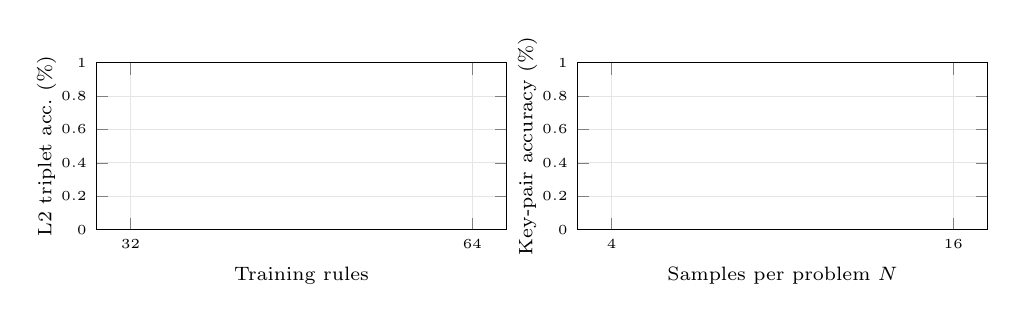
\begin{tikzpicture}
\begin{axis}[name=div, width=0.56\linewidth, height=3.7cm,
  xmode=log, log basis x=2, xtick={16,32,64,128,256},
  xticklabels={16,32,64,128,256},
  xlabel={Training rules}, ylabel={L2 triplet acc.\ (\%)},
  ymin=36, ymax=90,
  tick label style={font=\tiny}, label style={font=\scriptsize},
  ylabel style={yshift=-5pt}, grid=major, grid style={black!10}]
% <tables:fig-div>
% generated by scripts/make_tables.py (fig-div); do not edit
\node[red, font=\tiny] at (rel axis cs:0.5,0.5) {\ph{tbd}};
% </tables:fig-div>
\end{axis}
\begin{axis}[at={(div.east)}, anchor=west, xshift=9mm,
  width=0.56\linewidth, height=3.7cm,
  xmode=log, log basis x=2, xtick={1,4,16,64}, xticklabels={1,4,16,64},
  xlabel={Samples per problem $N$}, ylabel={Key-pair accuracy (\%)},
  ymin=48, ymax=88,
  tick label style={font=\tiny}, label style={font=\scriptsize},
  ylabel style={yshift=-5pt}, grid=major, grid style={black!10}]
% <tables:fig-seln>
% generated by scripts/make_tables.py (fig-seln); do not edit
\node[red, font=\tiny] at (rel axis cs:0.5,0.5) {\ph{tbd}};
% </tables:fig-seln>
\end{axis}
\end{tikzpicture}
\caption{Not yet measured; curves show the layout only. Left: L2 triplet
accuracy of \method{} as training grows by adding rules of new structures,
rules of structures already seen, or only cases for \ph{16} fixed rules (same
data size; bars: s.d.\ over seeds). Right: accuracy on both members of a
MedQA key pair for the trace selected among $N$ samples.}
\label{fig:diversity}
\end{figure}

\emph{Does a decision bit explain the rule-tier result?} If the reader also
writes whether the condition applies, a judge that sees only that bit and the
claim reaches \ph{tbd}\% on L2, against 99.2\% for the fact-only ledger. If the two
are close, the benefit on rules lies in what the reader is trained to
establish and not in the judge's use of the fields. Transfer is the other
test of the fields: \ph{38.2}\% against \ph{44.8}\% on MedEinst zero-shot
(Table~\ref{tab:ablation}), and a reader trained to write the bit without
fields reaches \ph{tbd}\%.

\emph{Own against program-supplied ledgers.} With program-supplied ledgers the
judge solves \ph{tbd}\% of L2 triplets. On the same items, \ph{tbd} errors of the full
model are rescued by the program-supplied ledger, \ph{tbd} correct judgments are
broken and \ph{tbd} errors are unchanged. The first number bounds what better
extraction could recover; it does not assign every error to the reader.
Applying the rule program to the predicted ledger gives \ph{tbd}\%, against 99.2\%
for the learned judge: if the program matches the judge, what the pipeline
contributes on executable rules is learning to extract applicable evidence.
Malformed ledgers are at most 0.17\% of records. A second pass that re-reads
each entry against the case and regenerates rejected ones gives \ph{tbd}\%.

\emph{One stage against two.} The one-stage variant, in which the ledger is
written as a rationale and the verdict is produced with the case in context,
solves 91.0\% of L2 triplets against 99.2\%. It is right on 99.6\% of
near-misses, so its deficit lies in reversal and not in holding
(reversal: \ph{tbd}\%). On MedEinst zero-shot it is \ph{2.7} points better than
the two-stage model: where a few typed fields cannot carry the evidence, the
bottleneck costs accuracy. With the prose record, a judge that also sees the
case reaches \ph{tbd}\% against 98.0\% without it.

\emph{Field interventions and the condition under test.} Changing
\texttt{subject}, \texttt{status} or \texttt{time} in a correct ledger changes
the verdict as the program prescribes in \ph{97.3}\% of cases, and given the
ledger of another case the judge returns the verdict that ledger implies in
\ph{96.8}\% (Appendix~\ref{app:ledger}). When the reader derives the condition
under test from the rule and the claim, triplet accuracy is \ph{tbd}\%.

\emph{Near-miss kinds not seen in training.} Trained on triplets from which
one kind of near-miss is removed, the verdict-only model solves \ph{tbd}\% of L2
triplets of that kind (another person), \ph{tbd}\% (past) and \ph{tbd}\% (threshold);
the applicability ledger \ph{tbd}\%, \ph{tbd}\% and \ph{tbd}\%. This tests whether near-miss
supervision has to enumerate the kinds, and whether a record helps where it
was not enumerated.

\emph{Rule diversity, model size, missing inputs.}
Figure~\ref{fig:diversity} (left; not yet measured): rules of new signature
classes raise L2 accuracy from \ph{tbd}\% to 99.2\%, rules of seen classes to
\ph{tbd}\%, more cases to \ph{tbd}\%. With the 4B model of the same family the
verdict-only model trained on blocks reaches 49.9\%, against 58.2\% for the
9B model; the other cells are not run, so we draw no conclusion about scale.
Missing-evidence rejection is at the ceiling for every trained model, since
the marker of a missing input is learnable from the 15\% of such records in
each corpus; we report this as a limit of that test and not as evidence of
abstention.

\subsection{Candidate selection}
\label{sec:results-downstream}

\begin{table}[t]
\centering\small
\setlength{\tabcolsep}{2.4pt}
\begin{tabular}{@{}lcccccc@{}}
\toprule
 & \multicolumn{2}{c}{Accuracy} & Key & \multicolumn{3}{c}{MedEinst}\\
\cmidrule(lr){2-3}\cmidrule(lr){5-7}
Selection & MQA & CQA & pair & pair & ctrl & trap\\
\midrule
% <tables:downstream>
% generated by scripts/make_tables.py (downstream); do not edit
Single sample & \ph{tbd} & \ph{tbd} & \ph{tbd} & \ph{tbd} & \ph{tbd} & \ph{tbd}\\
Self-consistency & \ph{tbd} & \ph{tbd} & \ph{tbd} & \ph{tbd} & \ph{tbd} & \ph{tbd}\\
Step check & \ph{tbd} & \ph{tbd} & \ph{tbd} & \ph{tbd} & \ph{tbd} & \ph{tbd}\\
\ \ \ vignette swapped & \ph{tbd} & \ph{tbd} & \ph{tbd} & \ph{tbd} & \ph{tbd} & \ph{tbd}\\
Ledger score & \ph{tbd} & \ph{tbd} & \ph{tbd} & \ph{tbd} & \ph{tbd} & \ph{tbd}\\
Combined & \ph{tbd} & \ph{tbd} & \ph{tbd} & \ph{tbd} & \ph{tbd} & \ph{tbd}\\
\ \ \ vignette swapped & \ph{tbd} & \ph{tbd} & \ph{tbd} & \ph{tbd} & \ph{tbd} & \ph{tbd}\\
\ \ \ no near-misses & \ph{tbd} & \ph{tbd} & \ph{tbd} & \ph{tbd} & \ph{tbd} & \ph{tbd}\\
\ph{Claude Opus 5.5} & \ph{tbd} & \ph{tbd} & \ph{tbd} & \ph{tbd} & \ph{tbd} & \ph{tbd}\\
\midrule
Oracle selection & \ph{tbd} & \ph{tbd} & \ph{tbd} & \ph{tbd} & \ph{tbd} & \ph{tbd}\\
% </tables:downstream>
\bottomrule
\end{tabular}
\caption{Reranking \ph{16} samples of a \bb{} policy on identical pools (\%).
MQA: MedQA; CQA: CareQA. Step check: injected-error PRM. Ledger score:
\method{} trained on rule triplets and clinical pairs. Combined: minimum of
the two after calibration.}
\label{tab:downstream}
\end{table}

Table~\ref{tab:downstream} tests the verifier as a process reward: selection
among samples of a fixed policy. It says nothing about a policy optimised
against the reward (Appendix~\ref{app:more}).
The combined reward and the step check improve accuracy on MedQA and CareQA
by similar amounts (difference \ph{0.7} [\ph{$-$0.2}, \ph{1.6}] on MedQA,
non-inferior at a margin of one point). On both members of a key pair the
combined reward reaches \ph{66.7}\% against \ph{58.9}\%, and on MedEinst pairs
\ph{45.9}\% against \ph{34.0}\%, with control accuracy unchanged. Swapping in
the vignette of another question removes the gain of the combined reward and
leaves the step check almost unchanged: the ledger score depends on the
supplied case. That the dependence is correct is what the pair columns show.
Without near-misses in training the combined reward loses \ph{1.2} points on
MedQA and nothing on MedEinst, whose pairs contain no near-misses. As $N$
grows, pair accuracy under the step check stays flat while the oracle rises
(Figure~\ref{fig:diversity}, right).

\section{Conclusion}

On executable rules, reward models fail in two directions. The remedy has two
parts: training with near-misses, and a record of what the case says, whose
it is and when, from which a case-blind judge decides. Trained on rules
alone, this carries to rules of unseen structure and, \ph{in part}, to
existing clinical labels. Holding on inapplicable evidence in clinical text
is not established.

\section*{Limitations}

\textbf{What the labels are.} Rule-tier labels establish compliance with a
stated rule, its applicability predicates and a rendering grammar. They say
what the rule implies, not what is clinically optimal, and that a program
produced a label does not show that the text expresses the state, that the
test is free of generator artefacts, or that the behaviour matters outside
the generator; these are addressed separately (Appendix~\ref{app:rules}). We
commissioned no new clinical annotation; reused benchmarks carry the review
their authors report. External results are agreement with released labels:
the TrialGPT annotations are physician judgments on synthetic patient
summaries, MedEinst cases derive from a simulator and were edited and
filtered by the benchmark, whose authors report physician review of
\ph{1{,}500} generated pairs, key pairs inherit the errors of exam keys and are
not counterfactuals, NLI4CT-P edits statements about breast-cancer trial
reports. Nothing here supports clinical use.

\textbf{The rule language.} The test is generated from a finite language of
applicability conditions (subject, status, time, thresholds). Held-out
signature classes reuse primitives and operators seen in training, there are
few such classes, and most judgments concern one condition of one rule: the
task is local applicability verification, not clinical reasoning. A trigger
lexicon that is given the test cue phrases solves the generated test, so its
difficulty lies in unseen wording and structure.

\textbf{Selectivity outside rules is tested only indirectly.} Applicability near-misses
with exact labels require a rule program. Beyond rules, holding is tested on
author-written cases and registered criteria, which still use our programs, and
on the claim side: by NLI4CT-P consistency under statement edits and by
expert-reviewed distractors in real discharge summaries that attribute a
correct fact to the wrong admission \citep{kim2026ehrnotechatqa}
(Appendix~\ref{app:qa}). No existing benchmark edits the case in this way;
assertion annotations of clinical notes \citep{uzuner2011i2b2} would allow a
test of the reader alone.

\textbf{The bottleneck.} The ledger assumes that a claim depends on a few
identifiable findings with a subject, status and time. Claims that weigh many
soft findings fit it poorly, and the one-stage variant is better on MedEinst.
The judge computes its verdict from the ledger; nothing guarantees that the
ledger is right, a quotation can exist in the case and still be the wrong
evidence, and hiding the case from the judge does not make its judgment
faithful. On the rule tier the condition under test is supplied.

\textbf{Verifier, process reward, training reward.} The triplet results
concern a claim verifier. Selection tests it as a process reward for one
policy. We do not show that a policy trained against it is safer, and we make
no claim about preventing reward exploitation beyond the policy-training
experiment.

\textbf{Rule population.} Rules come from our implementations of published
scores, constraints compiled from public recommendations and a grammar;
templates are cleaner than clinical notes. No clinician reviewed the rules.

\textbf{Development.} The generator and the systems were developed together,
and the frozen version followed an earlier one whose failure we describe in
Appendix~\ref{app:history}. Choices informed by earlier failures are listed
there.

\textbf{Weak supervision.} For rows trained on clinical pairs, ledger targets
come from differences between paired cases and from selection with a frozen
judge; they are not verified.

\textbf{Interpretation and scope.} The composition gap and shift classes are
descriptive. Measured values in this draft come from one seed and one
backbone. All data are in English.

\section*{Ethical Considerations}

The work uses public benchmarks and generated cases; no patient data were
collected. Stated rules in our data are test specifications and must not be
read as prescribing guidance. A reward model that appears to check patient
evidence could be trusted more than it should be; accuracy on these triplets
does not establish safety in care, and the models are released for research on
post-training only. Because the engine generates cases on which a given reward
fails, it could be used to construct inputs that mislead a deployed evaluator;
we see this as an argument for auditing rewards before they are used.

\bibliography{custom}

\appendix

\section{Analysis Plan}
\label{app:plan}

\ifplaceholders
\noindent\textcolor{red}{\textbf{Draft status.} Values printed in black
in the factorial, transfer, ablation, ladder and shortcut tables are measured
on \texttt{rule\_v1} with seed 0. Every value printed in red is a placeholder:
a number is a target value used to lay out an experiment that has not been
run, and ``tbd'' marks a cell with no value. Curves marked as placeholder
data are not measured. This paragraph and the red banner disappear, and the
build fails on any remaining placeholder, once measured values are
entered.}\smallskip
\fi

\noindent\textbf{Primary endpoints.} Triplet accuracy on L2 (rendered text,
rule stated) and reversal on MedEinst test pairs for the model trained on
rule triplets only.

\noindent\textbf{Primary comparisons} (paired on identical items, triplets
kept together, rules as clusters, Holm-corrected): on L2,
(1) balanced against natural, verdict only; (2) triplets against blocks,
verdict only; (3) applicability ledger against two-stage evidence summary,
triplets; on MedEinst, (4) rule-only \method{} against the untrained critic;
(5) rule-only \method{} against the rule-only evidence summary. Added before
any external result was seen: (6) on the TrialGPT annotations, the rule-only
model trained on triplets against the untrained backbone and against the
model trained on blocks.

\noindent\textbf{Decision rules.} If (2) fails, near-misses are reported as an
evaluation device only. If (3) fails, the paper is a data-design result and
the typed ledger is reported as equal to prose. If
(4) and (6) fail, the answer outside rules is negative and the medical claim
is withdrawn. If the gain in (4) appears
only with step-error data, it is reported as a gain from medical supervision.

\noindent\textbf{Status at seed 0.} (1) is not supported: balanced is below
natural. (2) holds by a wide margin. (3) is 1.2 points near the ceiling and
awaits the paired test. (4)--(6) are not run.

\begin{table}[!ht]
\centering\small
\setlength{\tabcolsep}{3pt}
\resizebox{\columnwidth}{!}{%
\begin{tabular}{@{}lcccc@{}}
\toprule
Comparison ($a-b$) & Diff. & 95\% CI & $p$ & $p_{\mathrm{Holm}}$\\
\midrule
% <tables:primary>
% generated by scripts/make_tables.py (primary); do not edit
(1) balanced $-$ natural, verdict only, L2 TA & -8.8 & [-11.9, -5.7] & \ph{tbd} & \ph{tbd}\\
(2) triplets $-$ blocks, verdict only, L2 TA & 33.1 & [29.6, 36.7] & \ph{tbd} & \ph{tbd}\\
(3) applicability ledger $-$ evidence summary, triplets, L2 TA & 1.2 & [0.2, 2.3] & \ph{tbd} & \ph{tbd}\\
(4) rule-only \method{} $-$ critic, MedEinst reversal & \ph{tbd} & [\ph{tbd}, \ph{tbd}] & \ph{tbd} & \ph{tbd}\\
(5) rule-only \method{} $-$ rule-only summary, MedEinst reversal & \ph{tbd} & [\ph{tbd}, \ph{tbd}] & \ph{tbd} & \ph{tbd}\\
(6a) \method{} triplets $-$ backbone, TrialGPT macro-F1 & \ph{tbd} & [\ph{tbd}, \ph{tbd}] & \ph{tbd} & \ph{tbd}\\
(6b) \method{} triplets $-$ blocks, TrialGPT macro-F1 & \ph{tbd} & [\ph{tbd}, \ph{tbd}] & \ph{tbd} & \ph{tbd}\\
% </tables:primary>
\bottomrule
\end{tabular}}
\caption{Primary comparisons (points). Paired on identical items; rules resampled
with their triplets (patients for TrialGPT); seeds paired by index; Holm over the
\res{cmp/holm/n} comparisons.}
\label{tab:primary}
\end{table}

\noindent\textbf{Selection and freezing.} Hyperparameters, thresholds, the
calibration of the combined reward and the choice of headline system use
development splits only: development triplets from training-fold signature
classes and a held-out part of the MedEinst reference set. Test sets are
generated or opened after these choices are frozen and are evaluated once.

\section{Rule Library and Splits}
\label{app:rules}

\begin{table}[!ht]
\centering\small
\setlength{\tabcolsep}{4pt}
\resizebox{\columnwidth}{!}{%
\begin{tabular}{@{}lrr@{}}
\toprule
Source & Rules & Classes\\
\midrule
% <tables:rules>
% generated by scripts/make_tables.py (rules); do not edit
Published scores, our implementation & 43 & --\\
Constraint rules from public recommendations & 60 & --\\
Grammar-sampled rules & 250 & --\\
MedCalc-Bench calculators            & \multicolumn{2}{r}{not included}\\
\midrule
Total (\texttt{rule\_v1}) & 353 & 21\\
% </tables:rules>
\bottomrule
\end{tabular}}
\caption{Rule population of the frozen library.}
\label{tab:rules}
\end{table}

\paragraph{What the labels establish.}
A program-derived label answers one of four questions
(Table~\ref{tab:validity}); the paper treats them separately.

\begin{table}[!ht]
\centering\small
\setlength{\tabcolsep}{3pt}
\begin{tabular}{@{}p{0.47\columnwidth}p{0.47\columnwidth}@{}}
\toprule
Question & Evidence\\
\midrule
Does the program implement the stated rule? & specification review by a second author; boundary, unit and dependency tests\\
Does the text express the intended state? & rendering audit by the authors (below); extraction check on rewrites\\
Does the test measure applicability and not artefacts? & shortcut scorers; rule-side items; author-written cases\\
Does the behaviour carry beyond the generator? & registered criteria; physician labels; MedEinst\\
\bottomrule
\end{tabular}
\caption{Four validity questions and the evidence for each.}
\label{tab:validity}
\end{table}

\paragraph{Manifest and provenance.}
The released manifest gives, for every rule, its source or specification, the
text shown in prompts, the program, its applicability semantics, its tests and
its version. Each rule is marked as a \emph{verbatim source rule} (\ph{tbd}), a
\emph{simplified source rule} (\ph{tbd}) or \emph{synthetic} (\ph{tbd}). Formalisations
of source-derived rules are checked against the source sentence by an author
who did not write them, because a generator that checks its own output can
repeat its own error; \ph{tbd} of \ph{tbd} were corrected or dropped. Requirements that
are ambiguous (for example ``adequate organ function'') are excluded and not
given an invented interpretation. We do not use the calculator set of
MedCalc-Eval \citep{mao2025medcalceval}, whose definitions were not available
to us. Because every prompt states the rule, correctness is relative to the
stated text for all sources.

\paragraph{Rendering audit.}
Before the freeze, 450 rendered groups were reviewed for label errors
\ph{[state who reviewed them and what they were asked]}; none was found in
base, flip, near-miss or presentation cases, and missing-input lines that
could be read as ``absent'' were reworded to ``unknown''. Presentation edits
that changed a fact, sampled alternatives ruled out by the condition, and
near-misses that differed from the flip in more than one attribute were found
and removed. The authors separately read \ph{tbd} groups for dropped negation,
wrong subject, ambiguous time expressions, conflicting measurements and
omitted exceptions, and found \ph{tbd}; this checks the rendering and not clinical
validity.

\paragraph{Constraint rules and claims.}
Each rule states a default option, a condition and an alternative. It is
derived from a public drug-label or guideline recommendation in three steps
taken from \citet{shen2026medguidex}, whose own functions are not released: a
model extracts the recommendation, writes it as a decision tree, and compiles
the tree to a program. We keep a rule if the tree is complete, the program
passes the boundary tests and agrees with the tree on sampled inputs, and
show the verbalised tree in the prompt. No clinician checks the tree against
the source, which is why labels are relative to the stated rule. Options
are plain orders of one form that differ by at most \ph{2} tokens and contain
no word that gives a reason. Every case reports the same fields with raw
values, so the presence of a field carries no label information.

\paragraph{Structure and complexity.}
Rule counts overstate variety, so Table~\ref{tab:structure} reports structure.
Most judgments concern one condition of one rule; where that is so we call
the task local applicability verification.

\begin{table}[!ht]
\centering\small
\resizebox{\columnwidth}{!}{%
\begin{tabular}{@{}lrr@{}}
\toprule
 & Train & L2\\
\midrule
Distinct program structures (names, constants removed) & \ph{tbd} & \ph{tbd}\\
Signature classes & \ph{tbd} & \ph{tbd}\\
Conditions needed per judgment (mean; max) & \ph{tbd} & \ph{tbd}\\
Dependency depth (mean; max) & \ph{tbd} & \ph{tbd}\\
Evidence mentions required (mean) & \ph{tbd} & \ph{tbd}\\
Cases with competing mentions of the concept (\%) & \ph{tbd} & \ph{tbd}\\
Judgments with a temporal operation (\%) & \ph{tbd} & \ph{tbd}\\
Judgments with a numeric comparison (\%) & \ph{tbd} & \ph{tbd}\\
Judgments with an exception (\%) & \ph{tbd} & \ph{tbd}\\
\bottomrule
\end{tabular}}
\caption{Structural statistics of \texttt{rule\_v1}.}
\label{tab:structure}
\end{table}

\paragraph{Splits and overlap.}
In each of \ph{3} folds \ph{5} of \ph{19} signature classes are held out for
L2. The levels change different things: L0 the generated cases only; L1 rule
identities and constants; L2 logical compositions; all test sets the wording.
Between training and L2 we report overlap of source documents (\ph{tbd}),
canonical programs (\ph{0}\%), parameter-normalised structures (\ph{tbd}),
criterion subexpressions (\ph{12.4}\%), rule texts (\ph{0}\%), rendering
templates and cue phrases (\ph{0}\%), and underlying states (\ph{tbd}): each input
type has \ph{6} templates, \ph{4} for training and \ph{2} for test, and the
words that mark relatives, negation and time are split in the same way. All
cases derived from one base state are in one split. With training templates
and cues on the same L2 rules, triplet accuracy of \method{} is \ph{tbd}, against
99.2\% with held-out ones. L3-alt moves one or two thresholds and keeps only
cases whose outcome differs between the original and the altered rule; its
near-miss kinds are \ph{tbd}, which is why models that fail on other kinds do
well on it.

\paragraph{Versions.}
\texttt{rule\_v1} was frozen, with hashes of every set, before the runs
reported here, and is not modified. Rule-side items, author-written cases,
rewritten cases and registered criteria are separate named sets, each frozen
before any system was scored on it. Defects found after the freeze are
listed with the affected items, and results are given with and without them
(\ph{tbd} items).

\section{Triplet Construction}
\label{app:twins}

\paragraph{Invariants.}
Every edit is checked on the target claim by executing the program: a flip
must change the claim, a near-miss and a presentation edit must not, also
for rules that combine criteria. Of the proposed flips, \ph{7.9}\% are
discarded because a second criterion changes or the claim does not; of the
proposed missing twins, \ph{18.6}\% because the remaining inputs determine
the claim. Near-misses are checked by executing the program on the state
recovered from the rendered case, and the equalities $h_k(x)=0$,
$h_k(\xf)=h_k(\xn)=1$ (or $h_k\equiv 1$ for measured inputs) are checked on
the rendered text of every triplet. Each training corpus has 60{,}000
records; L2 has 2{,}000 triplets and the development set 300. No evaluation
input contains the edit type, the role of the case, or the state.

\paragraph{Semantics.}
\emph{Several mentions.} A criterion uses the mentions its predicate counts;
for a measurement the most recent value dated at or before the reference
date, for a finding any counted mention with status present. A counted
``absent'' and a counted ``present'' for the same finding and time make the
state inconsistent, and such states are not generated.
\emph{Numbers.} Units are fixed per input and stated; where a unit conversion
is required it is part of the rule text. Thresholds are inclusive or
exclusive as the rule text says, and values exactly at a threshold form
their own near-miss kind. \emph{Time.} Every case has a reference date;
``within $W$ months'' includes the boundary day. \emph{Omission.}
Measurements that are not given are unknown; history items that are not
mentioned are absent, unless the case says they are unknown. This is a
stipulation of the generator, not a general reading of clinical notes; \ph{tbd}\%
of base cases state the required absence explicitly, and results on that
subset are \ph{tbd}. External datasets keep their own conventions.

\paragraph{Near-miss kinds.}
Numeric \ph{40}\% (of which at the threshold \ph{tbd}), other subject \ph{20}\%,
absent status \ph{20}\%, time outside the predicate \ph{20}\%. For criteria
whose predicate counts past or family findings, such mentions are flips.

\paragraph{Harder cases, by requirement.}
We do not use an undefined ``hard'' label. Table~\ref{tab:hard} lists the
requirements and how many test triplets have each.

\begin{table}[!ht]
\centering\small
\setlength{\tabcolsep}{3pt}
\begin{tabular}{@{}p{0.36\columnwidth}p{0.46\columnwidth}r@{}}
\toprule
Requirement & Example & $n$\\
\midrule
Rule-dependent time scope & the same past event counts under ``ever'', not under ``within six months'' & \ph{tbd}\\
Competing mentions & a relative has the finding; the patient explicitly does not & \ph{tbd}\\
Temporal selection & an older value crosses the threshold; the latest does not & \ph{tbd}\\
Composition & two conditions with an explicit exception & \ph{tbd}\\
Numerical semantics & values at inclusive and exclusive boundaries; unit given in the rule & \ph{tbd}\\
Long note & 15 or more unrelated lines & \ph{tbd}\\
\bottomrule
\end{tabular}
\caption{Requirements that define the harder cases.}
\label{tab:hard}
\end{table}

\paragraph{Rule-side items.}
For a fixed case, two rules differ only in the applicability clause: time
window, currency, subject, or boundary inclusivity. Each item has three cases
(the contested form, an uncontested positive, an absent finding) and is
solved only if all six judgments are right. A scorer that ignores the rule
text, one that never counts the contested form and one that always counts it
solve no item by construction (\ph{tbd} items; \ph{tbd} phrasings per clause).

\paragraph{Text tiers.}
\emph{Author-written cases}: \ph{tbd} groups written by the authors from state
specifications, each checked by a second author. \emph{Rewritten cases}:
notes rewritten by \ph{Gemma-3-27B} are accepted if two extractors recover
the intended state (\ph{8.7}\% rejected). Only accepted groups are scored
(\method{}: \ph{tbd}). Rejected rewrites may no longer express the intended state,
so their original label cannot be reused; they are kept as a data-quality
audit set and are not an evaluation set.

\section{External Tiers}
\label{app:qa}

\paragraph{Releases.}
MedEinst as released by its authors; NLI4CT-P as distributed for SemEval-2024
Task~2; MedPRMBench and CareQA at pinned revisions listed in the repository.

\paragraph{Registered eligibility criteria.}
Criteria are taken as written from registered trials (\ph{tbd} criteria from \ph{tbd}
trials). We keep single-condition criteria that can be decided from stated
facts: laboratory thresholds, events within a time window, current
conditions, pregnancy or breastfeeding, allergy, concurrent medication, age
bounds. For each we release the trial identifier, the exact text, whether it
is an inclusion or exclusion criterion, any normalisation, the program and
its boundary and time tests, and the reason for every exclusion. An author
who did not write the program checks it against the sentence; this is a
check of logic, not of medicine. Trials and criterion texts that occur in the
TrialGPT annotations are excluded. The set is used for testing only; training on such criteria would be a
separate experiment. Rule-side variants of a criterion are labelled as
synthetic interventions on the original text. Claims are ``The patient meets
this criterion'' and its negation.

\paragraph{TrialGPT annotations.}
The released file has 1{,}015 patient--criterion annotations over 53 patient
summaries and \ph{103} trials, with expert fields (eligibility label,
relevant sentences) and, separately, GPT-4 outputs. Protocol, fixed before
any system was scored: inputs are the patient summary as released and the
criterion with its type; no GPT-4 field is ever an input; targets are the
expert labels; the dataset's categories are kept, with ``not enough
information'' predicted when neither claim clears the acceptance threshold
carried over from the rule-tier development set, and ``not applicable''
items reported separately; the adapter and prompts are those selected on
rule-tier development data, and a patient-disjoint development portion
(\ph{tbd} patients) is used for interface decisions and excluded from the
reported test portion. The expert sentences evaluate evidence selection; they
do not validate the subject, status or time fields of a ledger. If eligibility
examples are later used for training, every compared method receives the same
added data. We report accuracy, macro-F1, class-wise errors,
and precision and recall of the reader's quoted sentences against the expert
sentences; intervals resample patients, and we inspect variation across
trials. The patient summaries are synthetic, so this is an external
expert-annotated evaluation, not validation on clinical records. Results:
backbone \ph{tbd}, verdict only with blocks \ph{tbd} and with triplets \ph{tbd}, matched
prose \ph{tbd}, \method{} with blocks \ph{tbd} and with triplets \ph{tbd} (macro-F1).

\paragraph{MedEinst.}
Claims are the two diagnoses. For training rows, the \texttt{found} targets
are the findings in which the two cases differ, taken from the structured
evidence where released and from a token diff otherwise; the two agree on
\ph{96.2}\% of a sample of \ph{500} pairs, and in \ph{97} of \ph{100} pairs
inspected by the authors the difference names the edited finding. Other ledger fields are not
supervised there. In the disease-held-out split a pair is in the test set
only if both of its diagnoses are test diseases (\ph{12} of 49), and in the
training set only if both are training diseases.

\paragraph{Key pairs.}
Pairs are mined within a split and reduced to a one-to-one matching, so that
no question occurs in two pairs. Excluded: negatively phrased lead-ins,
options that refer to other options, and questions without a case
description. For training rows, ledgers are sampled once from the frozen
rule-trained reader and kept if their quotations occur in the case and the
frozen rule-trained judge returns the keyed verdict on all four cells
(\ph{38.5}\% kept); the kept set is fixed and shared by all ledger formats. By
tercile of vignette similarity, reversal of the critic is \ph{55.7}\%,
\ph{44.1}\% and \ph{33.8}\%. CareQA covers six subject areas; results by area
are in the repository, and the biology and chemistry areas contribute
\ph{4}\% of pairs.

\paragraph{CondMedQA.}
CondMedQA \citep{parekh2026cgr} has 100 questions that contain a patient
condition, each with the answer given the condition and the general answer
that would hold without it; candidates were generated by a model, verified by
its authors, and 30 were reviewed by annotators with medical expertise. We
score both answers as claims for the question as posed and count how often
the condition-specific answer is preferred: \ph{41.0}\% for the critic,
\ph{56.0}\% for rule-only \method{} [\ph{46}, \ph{66}] and \ph{80.0}\% for the
closed judge. This is a test of resisting the default answer and not a
reversal pair, since the benchmark has no version of the question without the
condition; no rule is stated, so it also measures knowledge.

\paragraph{Claim-side applicability on real notes.}
EHRNote-ChatQA \citep{kim2026ehrnotechatqa} asks questions about a patient's
discharge summaries, each with one correct and four incorrect answers that
follow defined patterns and were reviewed by medical experts. Two patterns
mirror our near-misses on the claim side: a correct fact attributed to the
wrong admission, and a related entity or attribute taken from elsewhere in the
notes. Scoring each answer as a claim against the notes, the correct answer is
preferred to such a distractor in \ph{58.0}\% of cases by the critic, in
\ph{69.5}\% by rule-only \method{} and in \ph{77.0}\% with clinical pairs.
The data are under credentialed access and may not be sent to external
services, so closed judges are not evaluated on them.

\begin{table}[!ht]
\centering\small
\setlength{\tabcolsep}{3pt}
\resizebox{\columnwidth}{!}{%
\begin{tabular}{@{}lccc@{}}
\toprule
System & Key pairs & NLI-F & NLI-C\\
\midrule
% <tables:main-app>
% generated by scripts/make_tables.py (main-app); do not edit
\multicolumn{4}{@{}l}{\emph{Training-free, \bb}}\\
Critic & \ph{tbd} & \ph{tbd} & \ph{tbd}\\
\ \ + default correction & \ph{tbd} & \ph{tbd} & \ph{tbd}\\
\ \ + prompted ledger & \ph{tbd} & \ph{tbd} & \ph{tbd}\\
Generated-program verifier & -- & -- & --\\
\multicolumn{4}{@{}l}{\emph{Trained without medical QA data (clinical columns are zero-shot)}}\\
Verdict only, rule blocks & \ph{tbd} & \ph{tbd} & \ph{tbd}\\
Verdict only, FoVer data & \ph{tbd} & \ph{tbd} & \ph{tbd}\\
Verdict only, rule triplets & \ph{tbd} & \ph{tbd} & \ph{tbd}\\
Evidence summary, rule triplets & \ph{tbd} & \ph{tbd} & \ph{tbd}\\
GenPRM-style verifier, rule triplets & \ph{tbd} & \ph{tbd} & \ph{tbd}\\
\method{}, rule balanced & \ph{tbd} & \ph{tbd} & \ph{tbd}\\
\method{}, rule blocks & \ph{tbd} & \ph{tbd} & \ph{tbd}\\
\textbf{\method}, rule triplets & \ph{tbd} & \ph{tbd} & \ph{tbd}\\
\multicolumn{4}{@{}l}{\emph{With medical data}}\\
\method{}, rule triplets + step-error data & \ph{tbd} & \ph{tbd} & \ph{tbd}\\
\method{}, clinical pairs only & \ph{tbd} & \ph{tbd} & \ph{tbd}\\
\method{}, rule triplets + clinical pairs & \ph{tbd} & \ph{tbd} & \ph{tbd}\\
\multicolumn{4}{@{}l}{\emph{References}}\\
\ph{Claude Opus 5.5}, zero-shot & \ph{tbd} & \ph{tbd} & \ph{tbd}\\
\ph{Claude Opus 5.5}, prompted ledger & \ph{tbd} & \ph{tbd} & \ph{tbd}\\
Extraction + hand-written program & -- & -- & --\\
% </tables:main-app>
\bottomrule
\end{tabular}}
\caption{Rows of Table~\ref{tab:main} on key pairs (reversal) and NLI4CT-P
(faithfulness, consistency), \%.}
\label{tab:main-app}
\end{table}

\paragraph{NLI4CT-P.}
Base macro-F1 is \ph{71.0} for the critic and \ph{76.4} for rule-only
\method{}; joint correctness over an original statement and all its
interventions is \ph{38.5}\% and \ph{47.9}\%. Faithfulness and consistency follow the task definitions; pairs
that share an original statement are resampled together.

\paragraph{Overlap.}
By normalised question text, CareQA shares no question with MedQA. The MedQA
portion of ReMedQA \citep{cocchieri2026remedqa} lies within the MedQA test
split; we do not use ReMedQA.

\section{Ledger Format and Scoring}
\label{app:ledger}

{\footnotesize
\begin{verbatim}
need: penicillin allergy in the patient
found: "penicillin allergy (anaphylaxis)"
subject: other (mother)
status: present
time: current
\end{verbatim}}

\noindent Given this ledger, the rule and the claim ``Order amoxicillin'', the
judge returns \texttt{+}. Malformed ledgers occur in at most 0.17\% of rule-tier
and \ph{2.4}\% of MedEinst instances; a malformed ledger is recorded as an
invalid outcome and both claims are rejected. Neither record format may state
a verdict: on generated records a decision word or the text of a claim occurs
in \ph{tbd}\% of prose records and \ph{tbd}\% of ledgers. Temperature scaling for the combined
reward is fitted on development data separately for the two scores. The
verification pass prompts the same adapter with one ledger entry and the case
and asks whether value, subject, status and time are as recorded; it rejects
\ph{41}\% of wrong entries and \ph{3.2}\% of correct ones. In
triplet and pair evaluations one ledger serves both claims. In selection the
reader receives a step; for two candidate steps about the same criterion the
ledgers are identical in \ph{98.7}\% of cases. On L2 the reader is right on \ph{96.9}\%, \ph{95.4}\% and \ph{94.1}\% of
\texttt{found}, \texttt{subject} and \texttt{time} fields. In \ph{2.1}\% of
L2 cases it quotes a span that occurs in the case and is not the decisive
finding;
the string check cannot detect this.

\section{Diagnostics}
\label{app:diag}

\begin{table}[!ht]
\centering\small
\setlength{\tabcolsep}{4pt}
\resizebox{\columnwidth}{!}{%
\begin{tabular}{@{}lccc@{}}
\toprule
Scorer (L2) & Rev & Hold & TA\\
\midrule
% <tables:shortcuts>
% generated by scripts/make_tables.py (shortcuts); do not edit
Always default & 0.0 & 100.0 & 0.0\\
Claim only & 0.0 & 91.8 & 0.0\\
Concept named ($h_k$) & 46.6 & 0.0 & 0.0\\
Bag of words, case + claim & 13.2 & 61.7 & 7.0\\
Attribute-blind, logistic & 100.0 & 40.0 & 40.0\\
Trigger lexicon + program, training cue phrases & 96.7 & 57.3 & 54.0\\
\ \ given the test cue phrases & 99.5 & 100.0 & 99.5\\
General-purpose trigger tagger + program & \ph{tbd} & \ph{tbd} & \ph{tbd}\\
% </tables:shortcuts>
\bottomrule
\end{tabular}}
\caption{Shortcut scorers on L2 (\%); triplet accuracy measured. Entries of
the first three rows follow from Proposition~\ref{prop:blind}. Concept named:
any deterministic scorer that uses the case only through $h_k$.
Attribute-blind: a logistic model on concept--value features without subject,
status and time; it solves numeric triplets only. Trigger lexicon: a
rule-based reader with negation, experiencer and temporality triggers in the
style of ConText \citep{harkema2009context}, followed by the rule program.
Built from training cue phrases it reaches 54.0\%; given the test cue phrases
it reaches 99.5\%, which is a reference and not a baseline. The last row is a
frozen general-purpose implementation, which knows more synonyms than our
training phrases. Trained models that exceed these scorers outperform the
shortcut implementations tested here; this does not show that they use no
shortcut.}
\label{tab:shortcuts}
\end{table}

\begin{table}[!ht]
\centering\small
\setlength{\tabcolsep}{3.2pt}
\resizebox{\columnwidth}{!}{%
\begin{tabular}{@{}lcccccc@{}}
\toprule
Signal & Base & Ties & UR ($n$) & $P$ & $K$ & $G$\\
\midrule
Inj.-error PRM       & \ph{93.5} & \ph{0.0} & \ph{8.1} (\ph{4{,}769})  & \ph{92.8} & \ph{89.5} & \ph{71.4}\\
\bb{}           & \ph{80.2} & \ph{0.0} & \ph{24.6} (\ph{4{,}090}) & \ph{95.3} & \ph{91.2} & \ph{56.8}\\
Qwen3.5-27B          & \ph{88.4} & \ph{0.0} & \ph{26.0} (\ph{4{,}508}) & \ph{97.6} & \ph{95.4} & \ph{33.4}\\
\ph{Claude Opus 5.5} & \ph{96.0} & \ph{3.8} & \ph{12.9} (\ph{4{,}896}) & \ph{99.2} & \ph{98.1} & \ph{11.3}\\
\bottomrule
\end{tabular}}
\caption{L0 (\%). Base accuracy; tied preferences; unnecessary reversal among
triplets with a correct base preference, with its denominator; reading and
application reversal; composition gap.}
\label{tab:pk}
\end{table}

\paragraph{Near-miss decisions.}
Hold is near-miss correctness. To keep wrong-but-consistent decisions from
counting as desirable behaviour we also report, per system, the share of
base and near-miss pairs with the same decision, the share with both
decisions correct, and near-miss correctness given a correct base
(Table~\ref{tab:kinds}, with denominators per kind).

\begin{table}[!ht]
\centering\small
\setlength{\tabcolsep}{3pt}
\resizebox{\columnwidth}{!}{%
\begin{tabular}{@{}lccccc@{}}
\toprule
System & thr. & neg. & num. & subj. & time\\
\midrule
% <tables:kinds>
% generated by scripts/make_tables.py (kinds); do not edit
Verdict only, blocks & 33.8 & 93.2 & 92.0 & 11.5 & 60.5\\
\method{}, blocks & 72.0 & 97.5 & 99.8 & 48.5 & 58.8\\
Verdict only, triplets & 93.2 & 91.2 & 92.8 & 91.0 & 88.2\\
\method{}, triplets & 100.0 & 98.2 & 100.0 & 97.8 & 100.0\\
\midrule
$n$ (triplets) & 400 & 400 & 400 & 400 & 400\\
Same decision on base and near-miss & \multicolumn{5}{c}{\ph{tbd}}\\
Both correct & \multicolumn{5}{c}{\ph{tbd}}\\
Near-miss correct given base correct & \multicolumn{5}{c}{\ph{tbd}}\\
% </tables:kinds>
\bottomrule
\end{tabular}}
\caption{Triplet accuracy on L2 by near-miss kind (\%, seed 0): value at the
threshold, negated finding, value near the threshold, other person, past
finding. Lower rows: quantities to be reported per system.}
\label{tab:kinds}
\end{table}

\paragraph{Shift relative to a missing-input baseline.}
Let $d_0=d(\xm)$, $\delta(x)=d(x)-d_0$, and $y\in\{+1,-1\}$ the correct sign
of $d(x)$. For cases with $y\,d_0<0$, where the baseline preference opposes
the label, $y\,d(x)=-|d_0|+y\,\delta(x)$, so the preference is right if and
only if
\begin{equation}
y\,\delta(x) > |d_0| .
\label{eq:margin}
\end{equation}
Cases with $d_0=0$ have no opposing baseline and are counted separately. We
sort the others into four disjoint classes, in this order: \emph{crossed}
(Eq.~\ref{eq:margin}); \emph{unmoved} ($|\delta|\le\tau$, the model's median
$|d(x^{\mathrm{p}})-d(x)|$ over presentation edits); \emph{wrong direction}
($y\delta<0$); \emph{short}. The split restates the decision rule and adds the
direction and relative size of the shift. The \emph{shift ratio} compares that
size with the model's response to an error inside a step:
\begin{equation}
\kappa=\frac{\operatorname{med}\{\,y\,\delta(x): y\,d_0<0\,\}}
{\operatorname{med}\{\,u(s^{+},x)-u(s^{-},x)\,\}},
\label{eq:kappa}
\end{equation}
where the denominator runs over matched pairs of a correct step $s^{+}$ and
its injected-error version $s^{-}$ on the same case in the MedPRMBench
development split; both medians are in log-odds, and $\kappa$ is reported
with a bootstrap interval when the denominator is positive.
For the injected-error PRM, \ph{16.8}\% of baseline-conflicting cases cross,
\ph{55.2}\% move the right way and fall short, \ph{19.5}\% do not move and
\ph{8.5}\% move the wrong way; $\kappa=\ph{0.18}$
(Figure~\ref{fig:diagnosis}).

\begin{figure}[!ht]
\centering
\begin{tikzpicture}
\begin{axis}[name=tax, xbar stacked, width=0.60\columnwidth, height=3.5cm,
  xmin=0, xmax=100, bar width=5pt,
  ytick={1,2,3,4}, yticklabels={Verdict (blocks),27B judge,9B judge,Inj.\ PRM},
  ymin=0.4, ymax=4.6,
  tick label style={font=\tiny}, label style={font=\tiny},
  xlabel={Baseline-conflicting cases (\%)},
  legend style={font=\tiny, at={(0.5,1.04)}, anchor=south, legend columns=4,
                draw=none, /tikz/every even column/.append style={column sep=2pt}},
  legend image code/.code={\draw[#1] (0cm,-0.07cm) rectangle (0.2cm,0.07cm);},
  ymajorgrids=false, xmajorgrids, grid style={black!10}]
% <tables:fig-diag>
% generated by scripts/make_tables.py (fig-diag); do not edit
\node[red, font=\tiny] at (rel axis cs:0.5,0.5) {\ph{tbd}};
% </tables:fig-diag>
\end{axis}
\begin{axis}[at={(tax.east)}, anchor=west, xshift=9mm, ybar,
  width=0.42\columnwidth, height=3.5cm, bar width=5pt,
  ymin=0, ymax=1.3, ytick={0,0.5,1},
  symbolic x coords={Inj,8B,32B,Blk}, xtick=data,
  tick label style={font=\tiny}, label style={font=\tiny},
  ylabel={Shift ratio $\kappa$}, ylabel style={yshift=-5pt},
  enlarge x limits=0.2, ymajorgrids, grid style={black!10}]
% <tables:fig-diag-kappa>
% generated by scripts/make_tables.py (fig-diag-kappa); do not edit
\node[red, font=\tiny] at (rel axis cs:0.5,0.5) {\ph{tbd}};
% </tables:fig-diag-kappa>
\end{axis}
\end{tikzpicture}
\caption{Rule tier. Left: cases whose correct preference opposes the
missing-input baseline, by class (Eq.~\ref{eq:margin}; models that expose
log-probabilities). Right: shift ratio $\kappa$ (Eq.~\ref{eq:kappa}). Verdict
(blocks): the verdict-only model trained on flip blocks.}
\label{fig:diagnosis}
\end{figure}

\paragraph{Readouts and sampling noise.}
Dedicated PRMs use their released scoring head, open judges the log-odds of
the verdict token, and API judges without log-probabilities the verdict
frequency over \ph{32} samples at temperature \ph{1.0}, for which the standard
error of a frequency is at most \ph{0.09}. Scoring Qwen3.5-27B by the same
sampling protocol lowers its triplet accuracy from \ph{45.3}\% to
\ph{42.0}\%, with \ph{4.1}\% ties.

\paragraph{Input ablations.}
Replacing the question stem by ``No case description is available'' lowers
PRMScore on MedPRMBench by \ph{1.2}--\ph{2.9} points for trained PRMs. This is
an input ablation and not a measure of grounding: many injected errors are
detectable within the step, and chains restate patient facts. On the error
types that the benchmark defines relative to the case the loss is
\ph{4.0}--\ph{9.5} points, and \ph{6.2}--\ph{13.0} when numbers and quoted
spans of the stem are also masked in the chain.

\paragraph{Exploratory.}
A probe on the residual stream of the critic predicts the criterion outcome on
held-out signature classes with \ph{90.8}\% accuracy (control task
\citep{hewitt2019control}: \ph{49.6}\%); decodability does not show use
\citep{elazar2021amnesic}.

\section{Additional Results}
\label{app:more}

\begin{table}[!ht]
\centering\small
\setlength{\tabcolsep}{3pt}
\resizebox{\columnwidth}{!}{%
\begin{tabular}{@{}lccccc@{}}
\toprule
Variant (rule triplets only) & Rev & Hold & TA & MR & ME\\
\midrule
% <tables:ablation>
% generated by scripts/make_tables.py (ablation); do not edit
\method{} (facts only) & 99.2 & 100.0 & 99.2 & \ph{tbd} & \ph{tbd}\\
\ \ + decision field & \ph{tbd} & \ph{tbd} & \ph{tbd} & \ph{tbd} & \ph{tbd}\\
\ \ decision field only & \ph{tbd} & \ph{tbd} & \ph{tbd} & \ph{tbd} & \ph{tbd}\\
\ \ program on predicted bit & \ph{tbd} & \ph{tbd} & \ph{tbd} & \ph{tbd} & --\\
\ \ reader writes bit only & \ph{tbd} & \ph{tbd} & \ph{tbd} & \ph{tbd} & \ph{tbd}\\
\ \ condition derived by the reader & \ph{tbd} & \ph{tbd} & \ph{tbd} & \ph{tbd} & \ph{tbd}\\
\ \ + verification pass & \ph{tbd} & \ph{tbd} & \ph{tbd} & \ph{tbd} & \ph{tbd}\\
\ \ program-supplied ledger & \ph{tbd} & \ph{tbd} & \ph{tbd} & \ph{tbd} & --\\
\ \ program on predicted ledger & \ph{tbd} & \ph{tbd} & \ph{tbd} & \ph{tbd} & --\\
One-stage ledger & 91.3 & 99.6 & 91.0 & \ph{tbd} & \ph{tbd}\\
Value ledger & \ph{tbd} & \ph{tbd} & \ph{tbd} & \ph{tbd} & \ph{tbd}\\
Evidence summary (matched prose) & 98.5 & 99.3 & 98.0 & \ph{tbd} & \ph{tbd}\\
\ \ judge also sees the case & \ph{tbd} & \ph{tbd} & \ph{tbd} & \ph{tbd} & \ph{tbd}\\
Concept scorer & \ph{tbd} & \ph{tbd} & \ph{tbd} & \ph{tbd} & \ph{tbd}\\
Premise gate & \ph{tbd} & \ph{tbd} & \ph{tbd} & \ph{tbd} & \ph{tbd}\\
$-$ near-misses & 98.7 & 76.2 & 75.3 & \ph{tbd} & \ph{tbd}\\
\ \ + probe re-weighting & \ph{tbd} & \ph{tbd} & \ph{tbd} & \ph{tbd} & \ph{tbd}\\
$-$ other-person near-misses & \ph{tbd} & \ph{tbd} & \ph{tbd} & \ph{tbd} & \ph{tbd}\\
$-$ past near-misses & \ph{tbd} & \ph{tbd} & \ph{tbd} & \ph{tbd} & \ph{tbd}\\
$-$ threshold near-misses & \ph{tbd} & \ph{tbd} & \ph{tbd} & \ph{tbd} & \ph{tbd}\\
$-$ presentation edits & \ph{tbd} & \ph{tbd} & \ph{tbd} & \ph{tbd} & \ph{tbd}\\
$-$ ledger resampling & \ph{tbd} & \ph{tbd} & \ph{tbd} & \ph{tbd} & \ph{tbd}\\
Verdict only, pairwise loss & \ph{tbd} & \ph{tbd} & \ph{tbd} & \ph{tbd} & \ph{tbd}\\
% </tables:ablation>
\bottomrule
\end{tabular}}
\caption{Ablations on L2 and MedEinst zero-shot (\%); black: measured, seed 0.
Decision field: the reader also writes whether the condition applies.
Condition derived: the reader is given the rule and the claim and must find
the condition under test. Verification pass: every entry is re-read against
the case and regenerated once if rejected, after \citet{agand2026venra}.
Program-supplied ledger: the judge receives the target ledger; reported with
paired transitions in the text. Program on predicted ledger: the rule program
replaces the judge; it uses a program at test time. Concept scorer: fields
predicted by linear heads and a linear verdict. Premise gate: the step check,
attenuated toward a neutral score when the finding a step relies on is not
supported by a ledger extracted once per case, after \citet{evpv2026}. Probe
re-weighting: near-misses are not trained on; base--flip pairs whose
preference shifts under near-miss and presentation edits are down-weighted;
this is our adaptation of \citet{liu2026dynacf} to case edits, not a
reproduction. Rows that remove one near-miss kind are evaluated on triplets
of that kind. Pairwise loss: Bradley--Terry on the two claims.}
\label{tab:ablation}
\end{table}

\begin{table}[!ht]
\centering\small
\setlength{\tabcolsep}{3.2pt}
\resizebox{\columnwidth}{!}{%
\begin{tabular}{@{}lccccccc@{}}
\toprule
System & Dev & L0 & L1 & L2 & L3-inv & L3-alt & Long\\
\midrule
% <tables:ladder>
% generated by scripts/make_tables.py (ladder); do not edit
Critic & \ph{tbd} & \ph{tbd} & \ph{tbd} & \ph{tbd} & \ph{tbd} & \ph{tbd} & \ph{tbd}\\
Verdict only, blocks & 67.3 & 68.8 & 73.8 & 58.2 & 62.9 & 94.6 & 59.1\\
\method{}, rule blocks & 70.3 & 73.5 & 78.2 & 75.3 & 70.1 & 85.3 & 76.4\\
Verdict only, triplets & 99.7 & 99.0 & 97.6 & 91.3 & 96.9 & 100.0 & 90.5\\
\method{}, rule triplets & 99.7 & 99.7 & 99.1 & 99.2 & 97.9 & 100.0 & 98.3\\
Closed judge, ledger & \ph{tbd} & \ph{tbd} & \ph{tbd} & \ph{tbd} & \ph{tbd} & \ph{tbd} & \ph{tbd}\\
% </tables:ladder>
\bottomrule
\end{tabular}}
\caption{Rule ladder (triplet accuracy, \%); black: measured, seed 0. Dev:
trained rules, test wording; L3-inv: invented rules; Long: longer notes with
superseded values (requirements in Table~\ref{tab:hard}). On reading and
application pairs the first three trained systems reach 77.7\%, 76.0\% and
99.4\%. Macro-averages over rules and over signature classes, per-seed values
and the lowest held-out class are \ph{tbd}.}
\label{tab:ladder}
\end{table}

\begin{table}[!ht]
\centering\small
\setlength{\tabcolsep}{2.5pt}
\resizebox{\columnwidth}{!}{%
\begin{tabular}{@{}lcccccccc@{}}
\toprule
Run & s0 & s1 & s2 & s3 & s4 & Mean & s.d. & 95\% CI\\
\midrule
% <tables:seeds>
% generated by scripts/make_tables.py (seeds); do not edit
\texttt{B-F-ledger2-blocks} & 75.3 & -- & -- & -- & -- & 75.3 & -- & [72.0, 78.5]\\
\texttt{B-F-ledger2-triplets} & 99.2 & -- & -- & -- & -- & 99.2 & -- & [98.6, 99.7]\\
\texttt{B-F-rationale-blocks} & 61.5 & -- & -- & -- & -- & 61.5 & -- & [57.2, 65.5]\\
\texttt{B-F-rationale-natural} & 55.1 & -- & -- & -- & -- & 55.1 & -- & [50.1, 59.8]\\
\texttt{B-F-rationale-triplets} & 91.0 & -- & -- & -- & -- & 91.0 & -- & [87.9, 93.9]\\
\texttt{B-F-summary2-triplets} & 98.0 & -- & -- & -- & -- & 98.0 & -- & [97.0, 98.9]\\
\texttt{B-F-verdict-balanced} & 49.1 & -- & -- & -- & -- & 49.1 & -- & [45.6, 53.1]\\
\texttt{B-F-verdict-blocks} & 58.2 & -- & -- & -- & -- & 58.2 & -- & [54.2, 62.5]\\
\texttt{B-F-verdict-natural} & 58.0 & -- & -- & -- & -- & 58.0 & -- & [54.1, 61.9]\\
\texttt{B-F-verdict-triplets} & 91.3 & -- & -- & -- & -- & 91.3 & -- & [87.3, 95.0]\\
% </tables:seeds>
\bottomrule
\end{tabular}}
\caption{Triplet accuracy on L2 (\%) for every seed of every trained configuration
in the tables; -- marks a seed that was not run. Mean and s.d.\ over the seeds
run; the interval resamples rules with their triplets, seeds pooled.}
\label{tab:seeds}
\end{table}

\begin{table}[!ht]
\centering\small
\setlength{\tabcolsep}{3pt}
\begin{tabular}{@{}p{0.56\columnwidth}p{0.38\columnwidth}@{}}
\toprule
Comparison & Isolates\\
\midrule
Verdict vs.\ one-stage ledger & intermediate supervision\\
One-stage vs.\ two-stage ledger & separating reading from judgment\\
Two-stage ledger vs.\ matched prose & typed structure\\
Case-blind vs.\ case-visible judge & restricting access to the case\\
Own vs.\ program-supplied ledger & what better extraction could recover\\
Learned judge vs.\ rule program on the same ledger & what the neural judge adds\\
\bottomrule
\end{tabular}
\caption{Comparisons among interfaces and what each isolates.}
\label{tab:isolate}
\end{table}

\paragraph{Training.}
LoRA rank 64, batch size 64, one epoch over 60{,}000 records, learning rate
\ph{1e-4}, $\lambda=\ph{1.0}$, $p=\ph{0.3}$ \ph{[confirm against the run
manifest that ledger resampling was used]}. Rows with clinical pairs mix rule
triplets and pairs \ph{1}:\ph{1}. A verdict-only run takes about 2.2
GPU-hours and a two-stage run about 2.8, including evaluation; peak GPU
memory in the configuration with on-GPU checkpointing was 21.9~GB, which we
report for that configuration only.

\begin{table}[!ht]
\centering\small
\setlength{\tabcolsep}{3pt}
\begin{tabular}{@{}lccccc@{}}
\toprule
Configuration & Cases & Reader & Judge & Tokens & Steps\\
\midrule
Verdict only           & \ph{tbd} & -- & \ph{tbd} & \ph{tbd} & \ph{tbd}\\
Rationale              & \ph{tbd} & -- & \ph{tbd} & \ph{tbd} & \ph{tbd}\\
Evidence summary       & \ph{tbd} & \ph{tbd} & \ph{tbd} & \ph{tbd} & \ph{tbd}\\
Applicability ledger   & \ph{tbd} & \ph{tbd} & \ph{tbd} & \ph{tbd} & \ph{tbd}\\
\bottomrule
\end{tabular}
\caption{Supervision and compute per configuration: unique cases, reader
targets, judge targets, training tokens, optimiser steps. Equal record
counts do not by themselves mean equal supervision.}
\label{tab:budget}
\end{table}

\paragraph{Resources.}
Per scored claim: verdict only, \ph{1} pass and \ph{1} generated token;
\method{}, \ph{2} passes and \ph{45} tokens; generated-program verifier,
\ph{1} pass, \ph{540} tokens and one execution; GenPRM-style verifier,
\ph{1} pass, \ph{500} tokens and one execution; closed judge with ledger
prompt, \ph{1} API call and \ph{210} tokens, about \ph{60} times the list
price of the backbone per claim. Latency and hardware are in the repository.

\paragraph{Policy training.}
This is the only experiment in which a policy is optimised against a learned
reward, and the only basis for statements about reward exploitation. GRPO
from one \bb{} initialisation on rule triplets, \ph{3} runs, \ph{8}
rollouts per prompt, \ph{2000} steps, advantages standardised within a group.
Before each run we check that reward terms are not collinear within groups
and that the setup fits a \ph{64}-prompt subset. Accuracy on base--flip pairs
of held-out structures, judged by the rule program, moves from \ph{38.6}\% to
\ph{52.3}\% with an outcome reward, \ph{33.9}\% with the injected-error PRM
and \ph{63.5}\% with \method{}. A reference-graph reward after
\citet{medceg2025}, which scores a rollout by its coverage of the decisive
findings and of the chain from finding to criterion to conclusion, gives
\ph{58.0}\%; the rule program supplies the graph, so this reward, like the
outcome reward, uses the answer for each case.

\paragraph{Selection protocol.}
A trace is eligible if it contains a final answer (\ph{6.1}\% are not).
Ranking by the product of the two calibrated scores gives \ph{78.0}\% on
MedQA and \ph{66.1}\% on key pairs, a logistic combination fitted on
development data \ph{78.5}\% and \ph{67.0}\%, and the minimum \ph{78.3}\% and
\ph{66.7}\%. With
a paraphrased vignette the combined reward gives \ph{78.0}\% on MedQA. For
nested pools the selected reward cannot fall as $N$ grows, so we report
selection regret, the gap between oracle and selected accuracy: at $N=64$ it
is \ph{27.0} points for the step check and \ph{15.5} for the combined reward
on key pairs. On the open-ended version of CareQA, graded against reference
answers by a fixed model grader, the share graded correct moves from
\ph{48.2}\% to \ph{51.0}\%; this check is exploratory.

\section{Development History and Error Analysis}
\label{app:history}

\paragraph{The first generator and the shortcut it allowed.}
\ph{[Authors: write this from your own records.]} The pilot generator had 11
rules and three templates per mention form, shared between training and
development data. A verdict-only model trained on its triplets solved every
development triplet. On rules held out from training in which a past or a
family finding counts, it solved \ph{59.7}\%: with past and family mentions
never counting in training, ``past or family means ignore'' was a sufficient
strategy. This result is from the pilot setup and motivates the rule-side
test; it is not a failure shown for the current library.

\paragraph{What changed.}
\texttt{rule\_v1} holds out signature classes, templates and cue phrases;
contains rules under which past or family findings count; adds presentation
edits and missing inputs to every corpus; and was frozen before the runs
reported here. Rule-side items test the same failure directly and were built
after the freeze as a separate set.

\paragraph{Errors of the trained systems.}
From \ph{tbd} sampled failures, stratified by system and near-miss kind and
coded by the authors: extraction errors \ph{tbd}, applicability errors
\ph{tbd}, wording not seen in training \ph{tbd}, rule misread \ph{tbd},
other \ph{tbd}.

\ifplaceholders\else
\section{Reproducibility}
\label{app:repro}
Every number in this paper is produced by a script that writes the
corresponding table or figure. The rule manifest, the grammar, the triplet
engine, the key-pair miner, prompts, splits, model revisions and trained
adapters are released with the paper.
\fi

\end{document}
